\documentclass[a4paper,12pt,abstracton,titlepage]{scrartcl}
\usepackage{scrpage2}
\usepackage[utf8]{inputenc}
\usepackage[T1]{fontenc}
\usepackage[top=2.5cm, bottom=2.5cm, left=2cm, right=2cm]{geometry}
\usepackage[affil-it]{authblk}
\usepackage{lipsum}
\usepackage{url}
\usepackage[hidelinks]{hyperref}
\usepackage{graphicx}
\usepackage[table,xcdraw]{xcolor}
\usepackage{longtable}
\usepackage{multicol}
\usepackage[toc,page]{appendix}

% header
\pagestyle{scrheadings}
\setheadsepline{0.2pt}
\clearscrheadings
\automark[section]{chapter}
\ihead{D.S.C. Schiavini and M. Baertsoen}
\ohead{Useful feedback in the Ampersand parser}
\cfoot{\pagemark}

% code listings
\usepackage{listings}
\usepackage{color}

\definecolor{mygreen}{rgb}{0,0.6,0}
\definecolor{mygray}{rgb}{0.5,0.5,0.5}
\definecolor{mymauve}{rgb}{0.58,0,0.82}
\lstset{%
    basicstyle=\small\ttfamily,
    breakatwhitespace=true,          % sets if automatic breaks should only happen at whitespace
    breaklines=true,                 % sets automatic line breaking
    commentstyle=\color{mygreen},    % comment style
    keepspaces=true,                 % keeps spaces in text, useful for keeping indentation of code (possibly needs columns=flexible)
    keywordstyle=\color{blue},       % keyword style
    numbersep=5pt,                   % how far the line-numbers are from the code
    numberstyle=\tiny\color{mygray}, % the style that is used for the line-numbers
    stepnumber=1,                    % the step between two line-numbers. If it's 1, each line will be numbered
    stringstyle=\color{mymauve},     % string literal style
}

\lstnewenvironment{haskell}{\lstset{language=Haskell,numbers=left, otherkeywords={}, deletekeywords={}}}{}
\lstnewenvironment{adl}{\lstset{language=Haskell,numbers=left, otherkeywords={INCLUDE,CONTEXT,ENDCONTEXT,EXTENDS,THEMES,META,PATTERN,ENDPATTERN,PROCESS,ENDPROCESS,INTERFACE,CLASS,FOR,BOX,ROWS,TABS,COLS,INITIAL,SQLPLUG,PHPPLUG,TYPE,POPULATION,CONTAINS,UNI,INJ,SUR,TOT,SYM,ASY,TRN,RFX,IRF,AUT,PROP,ALWAYS,RULE,MESSAGE,VIOLATION,SRC,TGT,TEST,RELATION,MEANING,CONCEPT,IDENT,VIEW,ENDVIEW,DEFAULT,TXT,PRIMHTML,TEMPLATE,KEY,IMPORT,SPEC,ISA,IS,I,V,CLASSIFY,PRAGMA,PURPOSE,IN,REF,ENGLISH,DUTCH,REST,HTML,LATEX,MARKDOWN,ONE,BYPLUG,ROLE,EDITS,MAINTAINS}, deletekeywords={String}}}{}
\lstnewenvironment{ebnf}{\lstset{language=Haskell, numbers=none, otherkeywords={::=,=>}, deletekeywords={String}}}{}

\newcommand{\code}[1]{\texttt{\small #1}}

%citations
\usepackage{multibib}
\newcites{pr}{Project references}
\newcites{ac}{Academic references}
\newcites{nac}{Other references}

% code for generating glossary, from http://tex.stackexchange.com/a/5837/59718
\usepackage[acronym,toc]{glossaries}
\usepackage{glossary-mcols}
\newcommand{\dict}[2]{%
  \newglossaryentry{#1}{name=#1,description={#2}}%66
  \glslink{#1}{}%
}
\makeglossaries

% Here we set up the header, meta-information and front matter
%\date{November 3, 2014}      %// Today's date will appear when this is commented out.
\newcommand{\version}{Version 1.0}

% title page
\title{Useful feedback in the\\ Ampersand parser}
\subtitle{Gebruikersvriendelijke feedback in de Ampersand parser}
\titlehead{\centering\includegraphics[width=2cm]{Figures/AmpersandLogo}}
\author{
	Daniel S. C. Schiavini, Utrecht, Netherlands\\
	Maarten Baertsoen, Deinze, Belgium \\
  \normalsize
	~\\
  Student numbers 851102873 and 850044695\\
  ~\\
	Supervisor: Bastiaan Heeren\\
	Examiner: Marko van Eekelen}
\affil{Open Universiteit Nederland\\
    Faculteit Management, Science and Technology\\
	T61327 -- Afstudeerproject bachelor informatica} %\\
	%~\\\normalfont
	%\version}
% \publishers{\normalfont\normalsize\parbox{0.8\linewidth}{\textbf{Abstract}. \lipsum[1]}}

% URL's
\renewcommand*{\UrlFont}{\footnotesize\ttfamily}
\renewcommand*{\sectionautorefname}{Section}
\renewcommand*{\subsectionautorefname}{Subsection}
\renewcommand*{\subsubsectionautorefname}{Subsection}

% hyphenation
\hyphenation{
	cha-ra-cte-ris-ti-cs
	gua-ran-tee
	pro-duct
	cor-res-pon-ding
	me-cha-nism
	know-ledge
	de-ve-lo-pers
	do-cu-men-ta-tion
	sa-tis-fac-tion
	Schi-a-vi-ni
	Ba-ert-so-en}

% Now the document starts
\begin{document}
\maketitle
\newpage

\documentclass{article} % doesn't matter
\usepackage{pdfpages}
\begin{document}
\includepdf[pages={2-2}]{Thesis.pdf}
\end{document}
% !TEX root = ../Thesis.tex

% een korte samenvatting (plusminus 250 woorden)
\begin{abstract} 
Ampersand is een methode om businessregels een grotere rol te geven tijdens softwareontwikkeling.
Businessregels worden geschreven in scripttaal (ADL) en door Ampersand gecompileerd naar ontwerpartefacten, documentatie en prototypen.
Naarmate het project groter wordt, krijgen gebruikers steeds meer last van de slechte kwaliteit van de gegenereerde foutberichten.
Vooral nieuwe gebruikers worden hierdoor gehinderd en gefrustreerd.

Onze opdracht, gegeven door Prof.dr. Stef Joosten, is om betere gebruikersfeedback te ontwerpen en te implementeren.
Eerst hebben wij onderzocht wat goede berichten inhouden en hoe deze in Haskell geïmplementeerd worden, met de conclusie om de parser te herschrijven met Parsec.
Daarnaast hebben wij een onderzoek gevoerd naar het gebruik van businessregels en de Ampersand-aanpak.

De documentatie van de parser en de ADL-grammatica was niet up-to-date, waardoor wij reversengineering hebben toegepast om de documentatie vast te leggen.
Door refactoring hebben wij de leesbaarheid, uitbreidbaarheid, onderhoudbaarheid, documentatie en performance van de parser en de grammatica verbeterd, zonder de ADL-taal te beïnvloeden. 
Een automatisch testsysteem is geïmplementeerd met de mogelijkheid om de parsetree te `prettyprinten’ als ADL-code.

De nieuwe Ampersand parser is inmiddels geïntegreerd en in productie genomen.
Onze analyse toont aan dat de goede foutberichten van 22\% naar 82\% zijn gestegen, terwijl slechte fouten daalden van 56\% naar 1\%.

In deze presentatie laten wij zien hoe de nieuwe parser de doelstellingen behaalt en hoe deze verbeteringen het mogelijk maken dat Ampersand kan blijven groeien.
Deze verbeteringen zullen tijd en inspanning besparen voor studenten, onderzoekers en commerciële gebruikers.

~\\
\centering{
De presentatie zal gegeven worden op:\\
Dinsdag 30 juni om 13u15\\
~\\
Open Universiteit Nederland\\
Studiecentrum Utrecht\\
Vondellaan 202, 3521 GZ Utrecht
}

\end{abstract}

\clearpage

\tableofcontents
\listoffigures
\listoftables
\clearpage

% !TEX root = ../Parsing.tex
\section{Introduction}
\subsection{Identification}
This document contains the domain \& techniques analysis of the project `Useful feedback in the Ampersand parser'.
The document is the milestone product of the project phase 3a for Daniel S.C. Schiavini, as specified in the project planning \citenac{plan} \citeac{monadic-parsing}.

This document is part of the graduation project of the computer science bachelor at the Open Universiteit Nederland.
The project `Useful feedback in the Ampersand parser' is executed in collaboration with Maarten Baertsoen, with support of the supervisor Dr. Bastiaan Heeren and examiner Prof.dr. Marko C.J.D. van Eekelen.
The assignment is given by Prof.dr. Stef Joosten, who researches how to further automate the design of business processes and information systems by the development of the Ampersand project.

Ampersand is an approach for the use of business rules to define the business processes.
Users describe the business rules in a formal language (ADL), and Ampersand compiles those rules into functional specification, documentation and working software
prototypes.
The main objective of this project is to improve the feedback and maintainability of the Ampersand parser.
See \citenac{plan} for more details on the project.

\subsection{Goals}
The main objective of this phase is to gather information that will support the execution of the project.
This document contains the results of the research on domain and techniques that will support the project group.
It focuses on knowledge acquisition in two interrelated fronts:
\begin{description}
	\item[Haskell parsing libraries]
	In order to build the new Ampersand Parser (or refactor the current one), a research is done to choose the library best suited for the development.
	The appropriate library is chosen based on its design, documentation, features and generated errors.
	
	\item[User-friendly error messages]
	The most important feature of the parser that will be built, is that it should generate user-friendly error messages.
	To understand what kinds of messages can be (and should be) generated, a research will be done on what good errors are and how to generate them.
	This part of the research is done by consulting literature.
\end{description}
%
The results of both subjects culminate in a single section with research conclusions.

\subsection{Document overview}
An introduction is given is this section.
Then, in \autoref{sec:libraries} the choices of user-friendly error messages are elaborated.
In \autoref{sec:errors} the qualities of user-friendly error messages are briefly described, and in \autoref{sec:conclusion} the final conclusion is given.

Finally, in the appendix, a glossary of terms, definitions and abbreviations is given, just as a list of references.

\newpage
% !TEX root = ../Thesis.tex

%requirements plusminus 2 pagina's
\section{Objectives (M-R)}
\label{sec:objectives}
In this section we give an overview of the most important objectives of this graduation project, along with an introduction to the project and its context.
The complete list of objectives as given in the beginning of the project is given in the project planning \citepr{plan}.

\subsection{Ampersand project}
In November 2003, the Business Rules Manifesto \citenac{business-rules} was written, with the main purpose of declaring independence for business rules in the world of requirements.
The manifesto supports the vision of business rules as equivalent to requirements.
This is considered a radical change on how people see the world of business architecture.

In December 2010, Stef Joosten, Lex Wedemeijer and Gerard Michels published the paper `Rule Based Design', presenting the Ampersand approach.
The approach puts the rules in the center, using these rules to define the business processes.
Ampersand is named after the \& symbol with the desire of realizing results for both business and IT, in an efficient and effective way.

In 2011, the Ampersand compiler was created as an open source project.
Since then, the compiler has been improved and applied in both business and academic contexts.
The Ampersand end-users write business rules in a specific language (ADL), and compile that specification into functional specification, documentation and working software prototypes.
\dict{ADL}{Ampersand Design Language}%
These rules are based on agreements between the different stakeholders.

The theory behind Ampersand has been thoroughly studied, and is based on mathe\-matical concepts, e.g. relational algebra and Tarski's axioms.
Using this compiler, users write the requirements in ADL and generate all the system specification independent of the platform.
The main advantage is that the requirement's consistency and traceability are always correct (and even provable), from the lowest level up to the front-end.
The requirements are presented to stakeholders in natural language, guaranteeing that any business expert who knows the context can validate the requirements.
\autoref{fig:generation} depicts the artifacts generated by the Ampersand compiler.
%
\begin{figure}[htb]
	\centering
	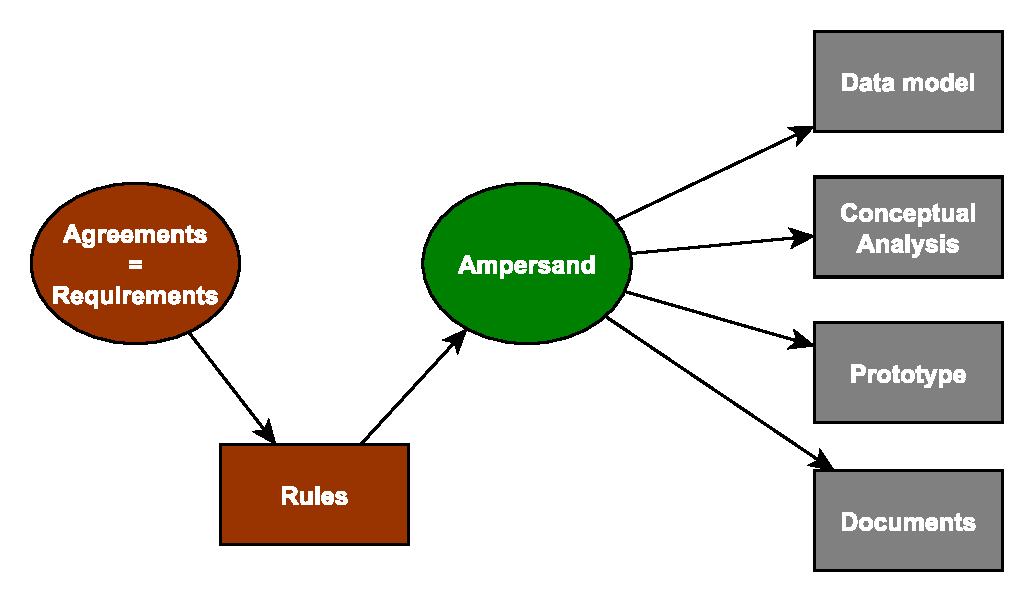
\includegraphics[width=0.7\textwidth]{Figures/Generation}
	\caption[Generated artifacts]{The Ampersand approach generates different artifacts based on the business rules (source: \cite{ampersand-approach})}
	\label{fig:generation}
\end{figure}
%

The Ampersand project is used in several environments, by different user groups.
In a research context, the Ampersand project is part of the research on the use of business rules for software design.
In an academic context, it is also used as the main tool in the course `Ontwerpen met bedrijfsregels' (code T18321) from the Open University of the Netherlands.
Finally, the compiler is used in business environments to design and develop real world business software.

\subsection{High-level architecture}
\label{subsec:architecture}
The compiler developed for the Ampersand research project runs in several steps, hence the Ampersand compiler is also divided in several subcomponents:
\dict{P-structure}{The parse-tree generated by the Ampersand parser, used as input for the type checker}%
\dict{A-structure}{The ADL code generated by the Ampersand type checker, used as input for the calculator component}%
\dict{ADL-structure}{See A-structure}%
\dict{F-structure}{The functional structure generated by the Ampersand calculator, used as input for the different output modules}%
\begin{itemize}
	\item \textbf{Parser}: This component receives the ADL code as input, and parses that code into a parse-tree (also known as P-structure).
	\item \textbf{Type checker}: The Ampersand type checker receives a P-structure as input and converts it into a relational algebra format, suitable for manipulation (also known as A-structure or ADL-structure).
		 The semantics of ampersand are expressed in terms of the A-structure.
	\item \textbf{Calc}: The Calc component receives an A-structure as input, and manipulates it according to the research rules, generating the functional structure (also known as F-structure).
		The F-structure contains all design artifacts needed to write a specification and generate the output.
	\item \textbf{Output components}: All design artifacts present in the F-structure are ready to be rendered.
		Several components use this data structure to generate the wished output.
		The output components currently implemented (and their output formats) are the following: 
		\begin{itemize}
			\item Atlas (HTML interface);
			\item Revert (Haskell source);
			\item Query (prototype generation);
			\item Documentation Generator (Pandoc structure).
		\end{itemize}
\end{itemize}

\subsection{User-friendly parser}
The end-to-end process of the ampersand project, from compiling towards the generated artifacts, is correct, however there is a major improvement topic identified in the first step, the parsing of the input scripts.

One of the main complaints from users is the quality of the errors generated by the Ampersand parser, making it hard for the end users to correct faulty ADL statements.
Since the beginning of the project, the parser subcomponent never received special attention, and it has not been analyzed for improvements.

In order to generate better, useful and to the point error messages, it is assumed that a complete refactoring of the parser will be necessary.
The main challenge is to choose the correct kind of architecture and libraries.
Note that discovering which errors are the most common and what user-friendly messages consist of, is an important part of the assignment.
At the beginning of the project, no list of undesirable error messages is available.
Therefore it was up to us, as a part of the project, to judge which error messages were good enough and which were undesirable.

\subsection{Other objectives}
While designing and implementing the new Ampersand parser, the following objectives were also important:
\begin{itemize}
  \item \textbf{Integration}: The new parser must interface with the remaining Ampersand modules.
    It must thus be implemented in Haskell.
  \item \textbf{Libraries}: Since different implementation options are available, it was important to choose the most suitable Haskell parsing framework.
  \item \textbf{Maintainability}: Well-written and maintainable code is a must for the Ampersand project, since it is an open-source project.
    The maintainability must be either maintained or improved; otherwise the parser is not to be taken into production.
  \item \textbf{Tests}: Testing the parser well was a task for this project.
    The suggestion is to use testing tools to improve the process, e.g. QuickCheck.
  \item \textbf{Pretty-printing}: This is important in order to test the parser.
\dict{HPC}{Haskell Program Coverage}%
\dict{Haddock}{Software documentation generator for the Haskell programming language}%
\dict{HLint}{Statical analysis software that suggests maintainability improvements}%
  \item \textbf{Tools}: Within the Haskell community, several tools are popular to verify code quality and generate documentation, e.g. HPC, Haddock and HLint.
  \item \textbf{Fixed syntax}: The new parser must process the same inputs as the previous parser.
  \item \textbf{Fixed parse tree}: The new parser must produce the same outputs as the previous parser.
    Any further changes must be applied to the rest of the Ampersand system.
\end{itemize}

During the project, some additional requirements have been identified:
\begin{itemize}
  \item \textbf{Git/GitHub}: The changed software had to be integrated into the GitHub Ampersand project.
    The development itself happened in a separate branch of a separate fork, so that deliveries could be merged in a smooth way.
    This was an especially hard requirement for us, since we had no experience with Git.
  \item \textbf{Cabal}: The building system for Haskell had to be maintained as the building platform.
  \item \textbf{EBNF}: The syntax of the Ampersand grammar was specified in EBNF notation but was not up-to-date.
    Any changes to the syntax had to be documented according with this notation.
    One option was to add the EBNF as comment in the source code in order to make clear that the complete grammar is implemented correctly.
\end{itemize}

On top of the project goals, we also wanted to help the university and other students with our results.
Finally, building up knowledge was also important for us (i.e. functional programming, Haskell, compilers, parsers, LaTeX, Ampersand, business rules and research in general).

\newpage
% !TEX root = ../Thesis.tex

\section{Domain \& techniques}
\label{sec:domain}
% !TEX root = ../Thesis.tex

%algemeen overzicht domeinen en technieken plusminus 2 pagina's
\subsection{Overview}
\label{domain:overview}
Before the actual parser work can start, it is imperative that the project team establishes a solid foundation of the existing system and the environment in which the system is used.
This phase of the project (domains \& techniques) is meant to assure that this knowledge is sufficiently gathered through individual research.
A set of relevant topics needed to support the team during the project execution is listed and allocated to the project team members.
The allocation was based on the aspect that Maarten took the more functional topics where Daniel addressed the more technical topics.
This way, both the domains and the techniques are well covered.

The research of Maarten was focused on the goals of the Ampersand approach as a whole, within the domain of formal specification techniques.
It focuses on the Ampersand vision, the methodology, the way Ampersand is used in practice and the future road-map of the Ampersand approach.
This is depicted in \autoref{domain:approach}.

Daniel investigated the domain of user friendly error messages and how to create them.
The second part of Daniel's research investigated the technical considerations to take into account while selecting a new parser.
Finally, based on the acquired insight, a new parser was selected to be proposed to our project customer.
His research is explained in \autoref{domain:parsing}.

% !TEX root = ../Thesis.tex

% individueel verslag onderzoek deeldomein en bijhorende technieken, plusminus 5 pagina's
% details van domein en technieken in relatie met het onderzoeksproject
% academische verantwoording gemaakte keuzen

\section{The Ampersand approach}
\label{domain:approach}
The research on the Ampersand Approach is done by Maarten Baertsoen.
The objective was to understand the vision of Ampersand in relation towards other formal methods within the same domain.
It focuses on the strengths and weaknesses of formal methods for defining business requirements.
The Ampersand approach is positioned within these formal methods based on the strengths and weaknesses of the different approaches. 

% !TEX root = ../Parsing.tex

\section{The Ampersand Methodology}
\label{sec:AmpersandTheory}

\subsection{Software requirements, the problem statement}

In 1976,  Dr. Thomas E. Bell investigated the domain of requirement engineering \citeac{SoftReqProbs}, sponsored by the Ballistic Missile Advanced Technology Center with the goal to determine the magnitude and characteristics of requirement-related problems in software engineering and to indicate what type of techniques could correct these issues. 
One of the main conclusions was that requirement errors were the most numerous and that these kind of errors are very time-consuming and, hence, costly to correct.
In his conclusion, Dr. Thomas E. Bel advises to use methods and techniques during the requirement engineering process to ensure consistency within and  between the requirements, such as the unique naming of objects and correct relations between the requirements themselves.
Iin addition, he stressed that the applied methods must aid the verification and validation of the requirements.
 
Although the research is ancient history from an IT point of view, the conclusion is actually still very relevant and therefore, methods and techniques to further improve the quality and consistency of the captured requirements are still a hot topic within the domain of requirement engineering.

An important classification of requirements is made by  Prof.dr. Stef Joosten \citeac{Joosten_derivingfunctional} and Prof. dr. Alex Borgida \citeac{JuretaBEM10}, into early phase requirements (the business requirements), and the late phase requirements (the functional specifications). 

\subsubsection{Formal functional specifications}
The initial focus to tackle the requirements issue, in which the research still continuous after 30 years, was on the functional specifications by the introduction of formal methods for functional specifications \citenac{Sommerville10}, which were based on a mathematical representation of the specifications resulting in the ability to analyze, validate and transform them into useful artifacts during the subsequent design and implementation phases. 

As described by  Luqi \& Goguen, J. A. \citeac{LuqiGoguen1997}, these formal methods for functional specifications had a positive impact on the reliability of the software development process, specifically for the purpose of specification analysis, transformation and verification \citeac{Clarke96formalmethods}.
This  reflects  in the elaboration of several mature formal methods.
The formal methods are categorized into two domains:

\dict{Z}{Formal specification notation zed}
\dict{VDM}{Vienna Development Method}
\dict{Larch}{Languages and Tools for Formal Specification}
\dict{LOTOS}{Language Of Temporal Ordering Specification}
\dict{RAISE}{Rigorous Approach to Industrial Software Engineering}

\begin{description}
	\item[Algebraic languages] describing the system in terms of types of data, mathematical operations on those data and their relationships, such as Z \citeac{Spivey89}, VDM \citeac{RISC3820} and Alloy \citeac{Jackson02}.
	\item[Model based languages] using mathematical sets and sequences to express the system specification as a system state model such as OBJ \citenac{Goguen93introducingobj}, Larch \citenac{Guttag93larch:languages} and LOTOS \citeac{BolognesiB87}.
	\item[Hybrid languages] combining features of both algebraic as model-based languages like RAISE \citeac{George03thelogic} and CafeOBJ, an enhancement of the OBJ language \citeac{DiaconescuFO03}.
\end{description}

\subsubsection{Business requirements}
\dict{RML}{Requirement Modeling Language}
Although the positive impact of the formal specification methods, it was recognized that these techniques were not sufficient. Concisely summarized by Prof. dr. Eric S. K. Yu and Prof. dr. John Mylopoulos \citenac{Understandingwhys}, the formal specification methods focus on the `whats' and the `hows' of the desired system without an understanding of the `whys' behind them. 

Within the social environment in which a software system will be introduced, several stakeholders have different goals,  business requirements, and based on these, they will express, often imprecise and inconsistent, expectations. Only by the correct understanding of their business requirements, to a feasible extend, the requirement engineers will truly feel the `whys' needed to derive the correct `whats' and `hows' to support these different goals.

Several early phase requirement modeling languages, RMLs, were introduced and typically included \citeac{JuretaBEM10}: 
\begin{description}
	\item[An ontology of requirements] describing the needed information to capture and the desired properties and behavior of of the to-be system, the view on the world from the perspective of the to-be system. This includes instances such as `Entity', `Activity' and `Assertion' \citenac{RMLRevisited}.
	\item[Modeling primitives,] to model the concepts and the relations within the ontology.
	\item[Methods,] sometimes automated, to verify consistency and to perform additional analysis to verify if the stated requirements will satisfy the business expectations.
\end{description}

\noindent
\dict{CML}{Conceptual Modeling Language}
\dict{Telos }{From the Greek word which means end; the object aimed at in an effort; purpose}
\dict{KAOS}{Knowledge Acquisition in autOmated Specification}
\dict{i*}{i star}
\dict{COTS}{Commercial Off The Shelf}


Early RMLs such as RML\citenac{RMLRevisited}, provided initial methods but suffered from drawbacks such as extensibility as the provided ontologies were rather fixed meaning that no new notions on par with the existing instances could be addressed. CML \citenac{CML} , which evolved to Telos \citeac{mylopoulos90telos}, contained already additional flexibility. 

KAOS \citeac{KAOS} introduced the notion of `stakeholder goal' where i* \citeac{yu97a} even differentiated between independent and interrelated, joint goals.
Further research to introduce the concept of goal priorities is ongoing for which a new abstract requirements modeling language `Techne' \citeac{JuretaBEM10} is designed, based on the CORE ontology for requirements \citenac{JuretaMF08}. Techne will provide the framework for new RMLs containing methods to compare candidate solutions and their compliance towards the business requirements, a feature that will come in handy as many software engineering projects nowadays includes COTS package based solutions.

\subsubsection{Limitations and frequent issues}
\label{sec:drawbacks}
Besides the significant improvements and their positive impact in software engineering projects, several striking drawbacks related to the use of formal methods are identified \citeac{Joosten_derivingfunctional, LuqiGoguen1997}:
\begin{description}
	\item[Communication] Communication between the business users and the requirement engineers based on the mathematical model is difficult as the business users are not used with mathematical notations. Although the functional specifications are analyzed to make sure they are consistent, it still offers no guarantee that the business requirements are consistent and transformed correctly into functional specifications as they cannot be correctly understood by the end users.
	\item[Typical experience and knowledge of developers] Software developers are not used to develop based on mathematical models, or even lack the skills of higher mathematics. It requires extensive training for these developers to understand the mathematical models and to develop efficiently in these kind of software projects.
	\item[Theoretical approaches] Many formal methods are theoretical and their appliance is demonstrated by means of very simplified example, but when they are effectively used in practice, the gap between theoretical specification and practical coding appears to be problematic, not to say impossible.
	\item[Agile development] Building a formal specification of a complete system is sometimes perceived as not flexible towards agile development techniques in which a system is engineered incrementally. 
	\item[Package based development] Many large software projects nowadays are using package based, COTS, solutions which are configured to fit the needs of the users. In such projects this package is mostly kept as standard as possible, meaning that no or little development is added and the functionalities of the package are used as implemented. In most commercial packages, no specific formal information is provided that allow the use of formal verification and validation techniques. The same goes for cloud solutions which are offered as-is without any, or only very limited, room for changes.
	\item[From business requirements towards functional requirements]Early and late phase requirement methods tend to focus on their specific domain, business of functional requirements, not many methods provide a means to verify the translation from business to functional requirements.
	\item[Supporting tools] Most formal methods don't have supporting tools making it very cumbersome to use them in larger scaled projects, even when there are supporting tools available, they often lack a suitable user interfaces due to which the practical use is threatened.

\end{description}


\subsection{The goals of the Ampersand Methodology}
   
The Ampersand Methodology was founded in 2007 by the inventor Prof.dr. Stef Joosten  \citeac{Joosten_derivingfunctional}, with the vision to provide an answer to several of the main drawbacks of using formal techniques  in software engineering (listed in section \autoref{sec:drawbacks}). 
The Ampersand Methodology is  developed to provide a method to unify the informal process of capturing the needs of users with the formal process of specifying an information system and to provide a formal translation method between both processes, including the necessary tools to ensure that the methodology is useful in real life projects.
Special attention is given to the transformation and verification of the business requirements into functional specifications.

Bottom line, the methodology presents the means to structure and present requirements in such a way that they can be validated by end-users as well as be interpreted unambiguously by system engineers after an automated transformation into functional specifications and design artifacts while the consistency between both is guaranteed.

The Ampersand Methodology addresses several goals to achieve this vision:
\begin{description}
	\item[Communication]  To assure that the stakeholders can correctly understand and validate their needs, the requirements must be documented in a natural language to enable them, without any requirement engineering knowledge, to validate the formal system requirements. On the other hand, the requirements must be structured into formal  functional specifications to make them useful during the actual software development phase and to benefit from the advantages of formal methods. 
	\item[Completeness]A software system in which not all requirements are supported is useless. The Ampersand language must be fully declarative, meaning that all the requirements must be supported in the method to assure that all business requirements, relevant to the subsequent software system, are accommodated correctly in the system specification.
	\item[Consistency]One of the main goals of the Ampersand Methodology is to guarantee consistency, each specified requirement must be applicable, and respected, to all processes in the context of this requirement. The methodology needs to provide the means to assure this consistency.
	\item[Traceability] The requirements must be traceable in such a way that end-users can trace  functions back to the stated business requirements, allowing them to fully understand to reason why these functions are defined.
	\item[Supporting tools] In order to facilitate the adoption of the Ampersand Methodology outside an academic environment, Prof.dr. Stef Joosten defined the additional goal that the Ampersand Methodology must be accompanied with supporting tools to support the requirement engineers and this by creating design artifacts to be used by the software developers.
\end{description}

\subsection{The Ampersand approach}
The Ampersand Methodology introduces a specific approach how to achieve the specified goals. The Ampersand Methodology can support different languages, a specific instance called `Ampersand Definition Language', ADL, is implemented to support the Ampersand Methodology.
The reasoning used to explain the achievement of the different goals is based on ADL.

\subsubsection{Communication}

One of the key differentiators of this approach is that the business requirements are presented towards the stakeholder in natural language while the system engineers can use functional specifications which are automatically transformed from the business requirements, assuring the functional specification is consistent with the business requirements.

The innovative aspect of the Ampersand methodology to achieve this goal is that the business requirements are  represented as `business rules' using relational algebra. A business rule must be seen as a business requirement in the form of an invariant to be satisfied by the business. The business rules are transformed in an automated way by an accompanying ADL tool, assuring the correctness of the functional specification based on the relational algebra of the business rules. Once the functional specifications are generated, the ADL tool will transform them back into the business rules for business user validation. When the re-translated requirements are then still correct for the end users, the system engineers have the assurance that the functional specifications are fully consistent with the business requirements. 

The use of natural language is further facilitated by the fact that it is not limited to a single specific language, it supports any language that satisfies a predefined set of axioms that can be used, making it possible to address each business user in his own language.

\subsubsection{Completeness}
Initial methodologies to define business requirements lacked the power to add new notions besides the pre-defined instances. ADL is designed as a purely declarative language to avoid this drawback. ADL features user specified rules, in relational algebra, design patterns, defined as sets of rules, contexts in which rules are applied and a signaling construct. In ADL, rules are specified without specific pre-defined actions to avoid that they become too narrow, compromising the declarative aspect of ADL.

\subsubsection{Consistency}
Expressing each business requirement as a business rule using relational algebra provides a mathematical foundation to check all rules against each other and to identify inconsistency between two or more business rules.  Checking each rule on his consistency towards the full set of defined business rules manually is quite demanding and would compromise the efficiency of the method on real life projects. 
The consistency check is therefore automated by the supporting tool.

\subsubsection{Traceability}
Business requirements have a one-to-one relationship with business rules offering traceability back from a specific rule, specification, to the business requirement making it possible for the end-user to correctly identify the reasons why the business rule was identified.

\subsubsection{Supporting tools}
The practical use of the Ampersand Approach is supported by a tool built in the functional programming language Haskell. 
This tool produces a wide range of functionalities and design artifacts to support the validation, consistency checks and the subsequent software development steps:
\begin{description}
	\item[Business rules and consistency issues] The inputted business rules in ADL are compiled and typed checked.
	This is realized by using the Swierstra's combinator package for the compiler \citeac{uu-doc}  and the AG-preprocessor by Dijkstra and Swiestra for the type-checker \citenac{MiddelkoopDS10}.
	\item[Data model]  Class diagrams and entity-relationships are created using the the GraphViz package \citenac{gansner2006drawing}. 
	\item[Service catalogue] All possible services on the defined classes and relationships, such as create, get, update and delete,  are specified formally. This formal representation together with the pre- and postconditions of the service make it possible that several developers can program the services independently of each other. 
	It is up to the requirement engineers to determine which services that need to be implemented.
	\item[Function point analysis] A function point analysis providing an insight on the complexity of the system to be built  is generated according to the IFPUG guidelines (\url{http://www.ifpug.org/}). This degree of complexity can be used to estimate the remaining system development effort taking into account the impact of the Ampersand tool as an accelerator
	\item[Software prototype] A remarkable aspect of the Ampersand tool is that it makes it possible to generate a working prototype. The prototype is generated as a web application and uses a MySQL database.
\end{description}
 
\subsubsection{Training}
Although the Ampersand Methodology, including ADL, is not yet widely adopted in the domain of requirement engineering, the methodology, including the supporting tools, is educated by the Open University of the Netherlands, course `Ontwerpen met bedrijfsregels'. A specific site is dedicated to the methodology, as well for self-tuition or co-development purposes.

\noindent




% !TEX root = ../Parsing.tex

\section{User-friendly error messages}
\label{sec:errors}

\subsection{Parsing errors}
When a parser is executed and is unable to recognize the input text, an error is raised.
The main problem when this happens, is that the parser cannot know for sure what the programmer meant to write.
Only the programmer can know exactly what the purpose of the invalid input was.

However, parsers should be able to recognize the most common errors, and support the user to correct them.
Spenke et al. \cite{error-recovery} discuss the following assumptions regarding parsing errors:
\begin{enumerate}
	\item An incorrect program is very similar to a correct one;
	\item An error is very soon followed by a correct piece of program;
	\item There are symbols (e.g. keywords) that are ommited quite rarely, while some less important symbols are more frequently ommited (e.g. semicolons);
	\item There are some very reliable symbols which most likely do not occur by accident, but always in an specific context (e.g. then being part of an if statement);
	\item  If an error cannot be corrected by deletion and/or insertion of a few symbols, the reason is often a complete, misplaced syntactic unit, such as a whole expression where only a single constant is allowed;
	\item A frequent reason for syntax errors is typing errors. In addition, similar basic symbols, such as round and square brackets may easily be confused.
\end{enumerate}

\subsection{User-friendliness}
There is no formal definition of what user-friendly error messages are.
Indeed, an expert programmer will expect to see more details than an unexperienced student.

Therefore, it may be very important to be able to finetune the errors shown.
The developers of the compiler may want details of the inner workings of the system (e.g. the parse tree).
Students, on the other hand, may just want to see the most likely cause of their mistake.

\subsection{Implications for the Ampersand parser}
\label{subsec:errors-ampersand}
The following items have been identified in the literature as important in the error messages generated by parsers:
\begin{description}
	\item[Location] When an error is detected, it is crucial to point out where in the input text the error has been found.
		If the location is incorrect, the user will have to search through his/her entire program to find the syntax error \cite{helium-parser,uu-doc,error-correcting,parsec}.
	\item[Production rules] Listing which product rules are applicable at that moment can help the user to choose the correct one \cite{helium-parser}.
		However, students have been reported to get overwhelmed by the huge list of terminals currently generated by Ampersand in the case of errors \cite{heeren-error}. 
	\item[Misspellings] Very often, errors happen because the users mistype keywords and/or symbols.
		Tokens that are invalid, but very close to valid input and often misspelled, should be recognized by the parser \cite{helium-parser,error-recovery}.
	\item[Error recovery] When an error occurs, it is appropriate that the parser is able to recover from that error.
		This way, the parser can continue analyzing the input \cite{error-correcting,error-recovery}.
\end{description}

% !TEX root = ../ResearchContext.tex

\section{Conclusion}
\label{sec:conclusion}
The Ampersand approach is situated within several research contexts, such as the Business Rule Approach and formal systems.
Additionally, the Ampersand Parser is part of a broader parser research context.
Our conclusion is that the new Ampersand parser has a very small influence in its research context for business rules.
This parser does not offer any new features or improvements to the language.
The largest influence of the project is commercial and educational by improving the user experience.
We expect that the new parser will allow commercial, research and educational users to do their work faster and more efficiently.



% !TEX root = ../Thesis.tex

% individueel verslag onderzoek deeldomein en bijhorende technieken, plusminus 5 pagina's
% details van domein en technieken in relatie met het onderzoeksproject
% academische verantwoording gemaakte keuzen

\subsection{Parsing Libraries \& Friendly Errors}
\label{domain:parsing}
The research on parsing library and user-friendly error messages was done by Daniel Schiavini.
The objective was to gather enough technical information to support the design and implementation of the new Ampersand parser.
It focuses on knowledge acquisition in two interrelated fronts: a search for the parsing library best suited for this project and defining what constitutes good error messages.

The first choice made was to use a combinator library, instead of a parser generator.
The main reason to avoid parser generators is that it is hard to generate useful feedback.
It was then made clear that besides generating good messages, those messages should also be customizable.
Considering the library design, documentation, features, generated errors and error customization, Parsec was judged to be the best suited library for the new parser.
This advice to use Parsec was accepted by the customer.

A list of important consideration points on developing good feedback has been collected through the literature.
Finally, other factors besides error messages are also very important for giving useful feedback.
One of the most important factors is that the documentation should be always kept available, up-to-date, clear and concise.

The complete research report is available as a separate document \citepr{parsing}.

\newpage
\documentclass[a4paper,12pt,abstracton,titlepage]{scrartcl}
\usepackage{scrpage2}
\usepackage[utf8x]{inputenc}
\usepackage[T1]{fontenc}
\usepackage[top=2.5cm, bottom=2.5cm, left=2cm, right=2cm]{geometry}
\usepackage[affil-it]{authblk}
\usepackage{lipsum}
\usepackage{url}
\usepackage[hidelinks]{hyperref}
\usepackage{graphicx}
\usepackage[table,xcdraw]{xcolor}
\usepackage{longtable}
\usepackage{multicol}

%citations
\usepackage{multibib}
\newcites{ac}{Academic references}
\newcites{nac}{Informal references}

% code for generating glossary, from http://tex.stackexchange.com/a/5837/59718
\usepackage[acronym,toc]{glossaries}
\usepackage{glossary-mcols}
\newcommand{\dict}[2]{%
  \newglossaryentry{#1}{name=#1,description={#2}}%
  \glslink{#1}{}%
}
\makeglossaries

% Here we set up the header, meta-information and front matter
%\date{December 16, 2014}      %// Today's date will appear when this is commented out.
\newcommand{\version}{0.3}

% title page
\author{Daniel S. C. Schiavini and Maarten Baertsoen}
\affil{Open Universiteit Nederland, faculteit Informatica \\
	T61327 - Afstudeerproject bachelor informatica}
\title{Research Context}
\subtitle{Useful feedback in the Ampersand parser\\
	~\\
	Phase 3b}
\publishers{Version \version}

% header
\pagestyle{scrheadings}
\setheadsepline{0.2pt}
\clearscrheadings
\automark[section]{chapter}
\ihead{Daniel S.C. Schiavini and Maarten Baertsoen}
\ohead{Parsing libraries \& error messages}
\cfoot{\pagemark}

% URL's
\renewcommand*{\UrlFont}{\footnotesize\ttfamily}

% Questions and answers
\newcommand{\question}[1]{\noindent\textbf{#1}\\}
\newcommand{\answer}[1]{#1\\}

% hyphenation
\hyphenation{
	gua-ran-tee
	pro-duct
	cor-res-pon-ding
	me-cha-nism
	know-ledge
	de-ve-lo-pers
	do-cu-men-ta-tion
	sa-tis-fac-tion
	Schi-a-vi-ni
	Ba-ert-so-en}

% Now the document starts
\begin{document}
\maketitle
\newpage

\tableofcontents
\clearpage

% !TEX root = ../Parsing.tex
\section{Introduction}
\subsection{Identification}
This document contains the domain \& techniques analysis of the project `Useful feedback in the Ampersand parser'.
The document is the milestone product of the project phase 3a for Daniel S.C. Schiavini, as specified in the project planning \citenac{plan} \citeac{monadic-parsing}.

This document is part of the graduation project of the computer science bachelor at the Open Universiteit Nederland.
The project `Useful feedback in the Ampersand parser' is executed in collaboration with Maarten Baertsoen, with support of the supervisor Dr. Bastiaan Heeren and examiner Prof.dr. Marko C.J.D. van Eekelen.
The assignment is given by Prof.dr. Stef Joosten, who researches how to further automate the design of business processes and information systems by the development of the Ampersand project.

Ampersand is an approach for the use of business rules to define the business processes.
Users describe the business rules in a formal language (ADL), and Ampersand compiles those rules into functional specification, documentation and working software
prototypes.
The main objective of this project is to improve the feedback and maintainability of the Ampersand parser.
See \citenac{plan} for more details on the project.

\subsection{Goals}
The main objective of this phase is to gather information that will support the execution of the project.
This document contains the results of the research on domain and techniques that will support the project group.
It focuses on knowledge acquisition in two interrelated fronts:
\begin{description}
	\item[Haskell parsing libraries]
	In order to build the new Ampersand Parser (or refactor the current one), a research is done to choose the library best suited for the development.
	The appropriate library is chosen based on its design, documentation, features and generated errors.
	
	\item[User-friendly error messages]
	The most important feature of the parser that will be built, is that it should generate user-friendly error messages.
	To understand what kinds of messages can be (and should be) generated, a research will be done on what good errors are and how to generate them.
	This part of the research is done by consulting literature.
\end{description}
%
The results of both subjects culminate in a single section with research conclusions.

\subsection{Document overview}
An introduction is given is this section.
Then, in \autoref{sec:libraries} the choices of user-friendly error messages are elaborated.
In \autoref{sec:errors} the qualities of user-friendly error messages are briefly described, and in \autoref{sec:conclusion} the final conclusion is given.

Finally, in the appendix, a glossary of terms, definitions and abbreviations is given, just as a list of references.

% !TEX root = ../ResearchContext.tex

\section{Short research}
\label{sec:research}
By investigating the requirements defined in the project planning \citenac{plan}, we identify here two contexts in which the new Ampersand parser is implemented.
First, we identify the Ampersand context, thus the research for the formal definition of business rules and the generation of documentation and software based  on it.
Second, we identify the parser context, thus the research for better user feedback in parsers.
In the following subsections each of the two contexts are described, including our findings during the literature research.

\subsection{Ampersand}
The Ampersand project has the ambition to offer a holistic methodology, including supporting tools, to support organizations during a software development project.
A new way of business requirements gathering, using natural language, is introduced by Ampersand.
%TODO: We have educational users too!
In this context, the Ampersand users are typically business analysts who don't necessarily have programming experience.
The goal of these users is to specify, sometimes complex, business rules in the most efficient way possible while still avoiding ambiguity.
To achieve their goals, the strictness of formal languages are a `necessary evil'.
Therefore, syntax errors can be very frustrating for the users.

Andrei Lapets \citeac{lapets2009improving} concludes that user accessibility has not been a priority in the design of formal verification systems.
He concludes that the syntax is often unfamiliar and/or introduces an entire new environment the user has to learn how to work with.
Finally, he points out that formal systems often offer a bottom-up structure that forces users to implement the complete set of assumptions in their research domain; this is made worse by the fact that usually few external libraries are available.

There are several measures that can be taken in order to improve the accessibility.
For example, the syntax should be familiar, simple and concrete \citeac{lapets2009improving}.
However, this project does not have any influence in the syntax.
The syntax of the ADL language is a given, so our influence is constrained to better user errors and development maintainability.

\subsection{Parsing errors}
Although the new Ampersand parser has no influence on the research for better user feedback in parsers, it is important to identify this context because it is of great importance for the project.
Our literature research was focused on the error messages for parsers implemented in Haskell, and then mainly the LL($k$) parsers built with the Parsec library, which was chosen during our domain and technique research \citenac{parsing}.

Parsec has extensive error messages; giving position, unexpected input, expected productions and general user messages.
The error messages are given in terms of high-level grammar productions and can be localized for different (natural) languages \citeac{parsec-fast}.
Special care must be taken when using backtracking (the $try$-function) in the parsec library, as it may negatively influence the error messages generated \citeac{parsec}\citenac{try-harmful}.

Swierstra and Duponcheel \citeac{swierstra1996deterministic} describe how automatic error correction can be implemented.
This automatic error correction was used in the previous Ampersand parser.
However, the shortcomings of error correction have been described in our techniques research \cite{parsing} so this possibility is not used in the new Ampersand parser.













% !TEX root = ../ResearchContext.tex

\section{Questions}
\label{sec:questions}
The following questions have been asked to a researched involved in the research, namely Lloyd Rutledge.
His answers are given after each of the questions.

~\\
\question{What are the largest user complaints when using Ampersand?}
\answer{~}

\question{Do users appreciate the error correction done by the previous parser?}
\answer{~}
  
\question{May better user feedback allow for a more efficient research on formal business rules?}
\answer{~}

\question{Has the maintainability of the previous parser been an issue in our research?}
\answer{~}
  
\question{How can a new Ampersand parser, and a better user feedback, support the objectives of the Ampersand project?}
\answer{~}

\question{Ampersand is nu reeds een antwoord op gekende issues van toepassing op methodologien mbt business requirements (praktische bruikbaarheid, volledigheid, gebruik van natuurlijke taal, opleiding, ...) Tevens staan bijkomende uitbreidingen op de agenda (agile, responsive UI op basis van een repository,...)\\
Wat zijn volgens jou (Stef) de komende uitdagingen die eraan komen en wat is de visie hoe Ampersand daarin past?\\
--> bijvoorbeeld: nu wordt er gebruik gemaakt van natuurlijke taal die volgens een vaste grammatica verwerkt wordt, de kennis en achterliggende IT processen om natuurkijke taal te interpreteren volgens midner strikte structuren wordt alsmaar sterker, kan het een evolutie zijn om al een interpretatie te doen op bbasis van gesproken tekst (ter vorming van de basis)}
\answer{~}

\question{Ampersand is reeds sterk en zal alsmaar sterker worden, wat is de visie en aanpak hoe Ampersand verder in de 'markt' gepositioneerd zal worden?}
\answer{~}

\question{Is er de intentie om Ampersand te commercialiseren? Of, minder financieel gefocust, in een soort vzw onder gebracht van waaruit een (semi) professionele support gegeven kan worden aan de methodologie en tools (cfr PMI, ITIL,…)}
\answer{~}

\question{Waar kunnen we binnen het ABI project rekening mee houden om de toekomstvisie van Ampersand te ondersteunen? (maintainability van de code is bv al 1 aspect)}
\answer{~}

\question{De drempel om bij te dragen aan de Ampersand tools is eerder hoog: Los van de methode is er ook de praktische utiwerking. Haskell is op zich al geen courante en eenvoudige taal, en de uitwerking is bij momenten behoorlijk complex. Gezien het open-source aspect en de ambitieuze roadmap: wat is de visie om contributors aan te trekken en effectief hun weg te laten vinden in de code, project...}
\answer{~}

\question{Er bestaan reeds een aantal parsers, nu gaan we Parsec inbouwen, maar de kans is zeker bestaande dat er binnen x aantal jaar opnieuw geavanceerdere parsers uitgewerkt zullen worden, wat is de visie hoe we deze evolutie momenteel al kunnen supporteren? Zal Ampersand in de toekomst, afhankelijk van de context, de mogelijkheid moeten bieden om verschillende parsers toe te passen (bv via een selectie in een menuitem)}
\answer{~}

\question{Mogelijke onderzoeksvraag: Formele talen beloven een vorm van zekerheid op het vlak van correctheid, maar hoe correct de software ook is, fouten met oorsprong in analyse en het achterliggende redeneren kunnen een perfect formeel model vormen, zonder het gewenste resultaat. De Focus van ampersand ligt op het faciliteren van het beredeneren tijdens de analyse fase. Kan een betere foutafhandeling in ampersand ertoe bijdragen dat dit aspect binnen formele talen beter afgedekt wordt en formele talen niet enkel een juist maar ook een gewenst resultaat bekomen.}
\answer{~}

\newpage
% !TEX root = ../ResearchContext.tex

\section{Conclusion}
\label{sec:conclusion}
The Ampersand approach is situated within several research contexts, such as the Business Rule Approach and formal systems.
Additionally, the Ampersand Parser is part of a broader parser research context.
Our conclusion is that the new Ampersand parser has a very small influence in its research context for business rules.
This parser does not offer any new features or improvements to the language.
The largest influence of the project is commercial and educational by improving the user experience.
We expect that the new parser will allow commercial, research and educational users to do their work faster and more efficiently.



\part*{Appendices}
\addcontentsline{toc}{part}{Appendices}
\appendix
% !TEX root = ../ResearchContext.tex

\small
\printglossary[style=mcolindex,title=Glossary]
\label{sec:glossary}

\newpage
% !TEX root = ../Planning.tex
\addcontentsline{toc}{section}{References}
\label{sec:bibliography}

\begin{thebibliography}{99}

%TODO: Check the order of the bibliography

\bibitem{business-rules}
	The Business Rules Manifesto\\
	Version 2.0, November 1, 2003\\
	Ronald G. Ross\\
	\url{http://www.businessrulesgroup.org/brmanifesto.htm}
	
\bibitem{ampersand-approach}
	Ampersand: foutvrije specificaties voor B\&I-vraagstukken\\
	Informatie magazine, August 2007\\
	Stef Joosten, Rieks Joosten and Sebastiaan Joosten\\
	\url{http://informatie.nl/Artikelen/2007/augustus/Default.aspx}  % AmpersandfoutvrijespecificatiesvoorBI-vraagstukken.aspx
	
\bibitem{ampersand-architecture}
	Ampersand Software Architecture\\
	\url{http://wiki.tarski.nl/index.php/Software_Architecture}
	
\bibitem{pmi}
	Project Management Institute\\
	\url{http://www.pmi.org}
	
\bibitem{open-issues}
	Requirements for a parser of Ampersand\\
	Stef Joosten\\
	Version \texttt{8e27daf}, September 25, 2014\\
%	{\footnotesize \url{https://github.com/AmpersandTarski/ampersand/tree/ABI\_Parser/ArchitectureAndDesign}}
	\url{https://github.com/AmpersandTarski/ampersand/commit/8e27daf}
	
\bibitem{ampersand-wiki}
	Ampersand Coding Conventions\\
	Stef Joosten \& Han Joosten\\
	Version 4, September 6, 2011\\
	\url{http://wiki.tarski.nl/index.php/Coding\_conventions}.

\bibitem{heeren-error}
	Top Quality Type Error Messages\\
	Bastiaan Heeren\\
	ISBN 90-393-4005-6, September 20, 2005\\
	\url{www.open.ou.nl/bhr/phdthesis}.
	
\bibitem{iso-9126}
	Software Engineering -- Product quality\\
	International Organization for Standardization\\
	ISO/IEC 9126:2001\\
	\url{http://www.iso.org/iso/iso_catalogue/catalogue_tc/catalogue_detail.htm?csnumber=22749}.

\bibitem{jstd-016}
	J-STD-016 Standard for Software Development and Documentation\\
	Annex F.2.4: Contents of the Software Requirements Specification (SRS)\\
	Department of Defense, United States of America\\
	September 1995\\
	ISBN 0-7381-0427-2, SS94377.

\end{thebibliography}

\end{document}
\newpage
% !TEX root = ../Thesis.tex

\section{The previous parser}
\label{sec:analysis}
In this section, we analyze the previous Ampersand parser in order to understand its workings and signal the improvement points.
% !TEX root = ../Documentation.tex

\subsection{System overview}
\label{design:system-overview}
  The parser module overview is given in \autoref{fig:ParserModules}.
  \begin{figure}[ht]%
    \centering
    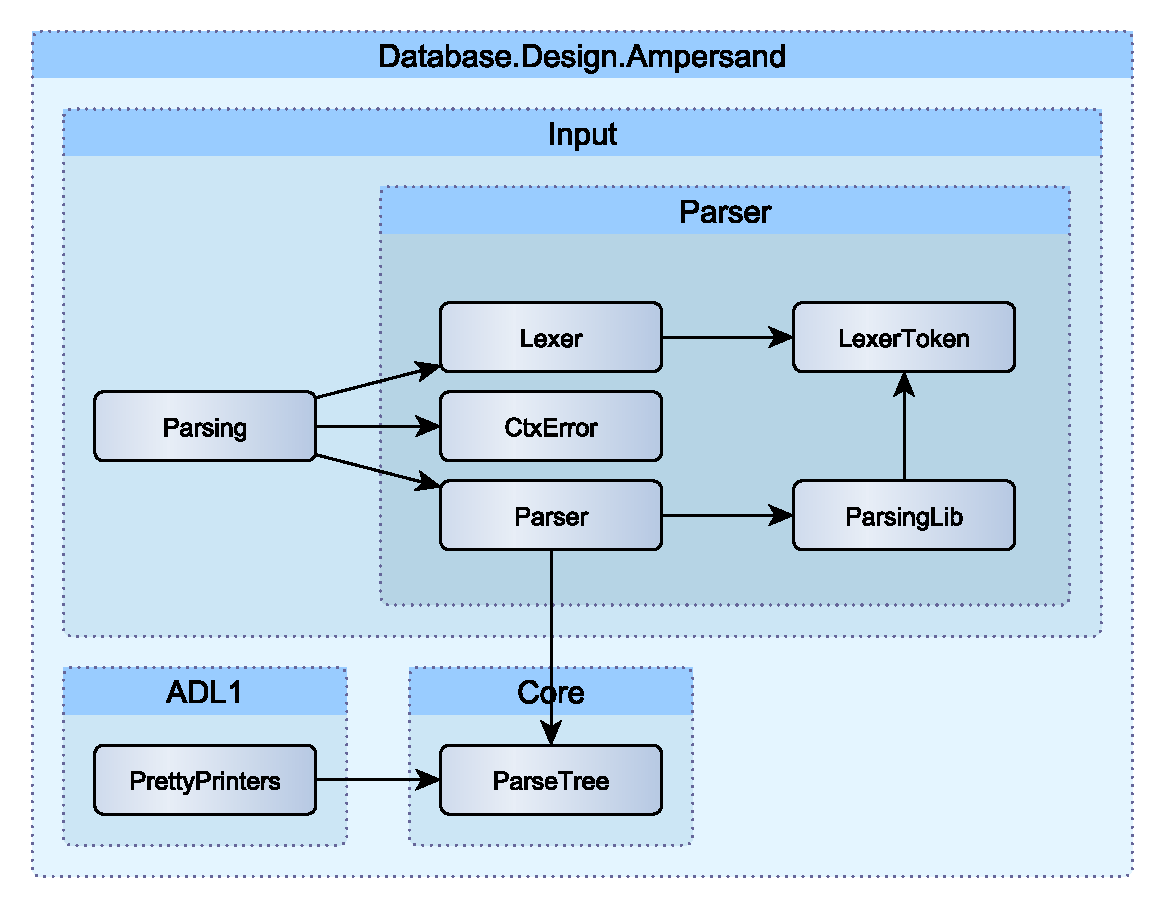
\includegraphics[width=0.7\columnwidth]{Figures/ParserModules}
    \caption{The modules relevant for the parser and their dependencies}
    \label{fig:ParserModules}
  \end{figure}%

  The parsing process starts in the module \code{Parsing}.
  As a first step, the input string is sliced into tokens by the \code{lexer} module.
  Once the input string is separated into the token structure as defined in the module \code{LexerToken} the next step is to actually parse the tokens by the \code{Parser}.
  The parser will use the \code{ParsingLib} to create the parse tree as defined in \code{ParseTree}.

  ~\\\noindent
  Each main module has the following responsibilities:
  %
  \begin{description}
    \item[Parsing] module that implements the interface of the parser with the rest of the system.
      It is responsible for reading the input files, calling the lexer and the parser and returning a parse tree as result (or a parse error).

    \item[Lexer/LexerToken] modules responsible for recognizing the input characters and converting them to tokens.
      The new lexer, together with its sub-modules, splits the input strings into the token structure defined in \code{LexerToken}.
      This list of tokens is the actual input for the parser.

    \item[Parser] module responsible for executing the parsing itself.
      It accepts the tokens that are allowed in each grammar production and generates the corresponding parse tree.
      The parser is described in \autoref{design:new-parser}.
 \end{description}

  \noindent
  Several supporting modules are defined used by one or more main modules:
  \begin{description}
    \item[ParsingLib] library that contains several useful functions to assist the parser, e.g. token recognition.
      These functions are not depending on the specific grammar rules.
      
    \item[ParseTree] external module containing the parse tree data structures.
      Only details of this module have been changed during this project (e.g. field ordering).
    
    \item[PrettyPrinters] contains instances of the \code{Pretty} type class for the parse tree data types and the functions responsible for printing the parse tree to ADL scripts in a `pretty' way.

    \item[CtxError] contains the data structures responsible for the parse errors and their location.
      This module has not been refactored as a part of this project.
    
  \end{description}

% !TEX root = ../Parsing.tex

\section{User-friendly error messages}
\label{sec:errors}
The most important feature of the parser that will be built, is that it should generate user-friendly error messages.
To understand what kinds of messages can be (and should be) generated, a research will be done on what good errors are and how to generate them.

This is also related to the choice of the parsing library, since the chosen library should support the generation of good errors without extensive effort.
Coincidently, a good source of knowledge are the papers of the supervisor, Bastiaan Heeren, who has done his PhD thesis on the generation of top quality type error messages\cite{heeren-error}.

% !TEX root = ../Thesis.tex

\subsection{Lexer}
\label{analysis:lexer}
The lexer module is responsible to split up the input stream into tokens.
Tokens are meaningful pieces of the input string that can be recognized by the parser.

The following improvement points were identified after analysis:
\begin{description}
  \item[Dispersed error messages]
    The error messages produced by the lexer are of good quality.
    Each error message is however defined directly within the corresponding lexer function making the maintenance harder.
  \item[Complex token structure]
    The token structure is complex and confusing.
    Two values are present in the token, of which one \texttt{val1} is never used.
    There is no distinction between the values used to identify the content of the token and the ones to determine the position of the token.
  \item[Module structuring]
    In the lexer, the actual lexing functions are intermingled with data types, supporting functions and error message texts.
    This makes the lexer hard to understand and to maintain.
  \item[Language support]
    The errors are returned in English only, no multilingual support is available.
  \item[No support for warnings]
    The lexer can only return errors, warnings are not supported. 
  \item[Strings only]
    Token values are stored as strings for all types, with no conversion of integer values.
  \item[Lacking documentation]
    There was no documentation available on how the lexer was designed and structured.
\end{description}


\subsubsection{Token structure}
The old token has the following structure:

\begin{verbatim}
data Token = Tok { tp' :: TokenType
                 , val1 :: String
                 , val2 :: String
                 , pos :: !Pos
                 , file :: !Filename
                 }

data TokenType
  = TkSymbol
  | TkVarid
  | TkConid
  | TkKeyword
  | TkOp
  | TkString
  | TkExpl
  | TkAtom
  | TkChar
  | TkInteger8
  | TkInteger10
  | TkInteger16
  | TkTextnm
  | TkTextln
  | TkSpace
  | TkError
  deriving (Eq, Ord)
\end{verbatim}
%
The arguments have the following purpose:
\begin{description}
  \item[TokenType]
    Identification of the token type. %, i.e. \texttt{TkSymbol}, \texttt{TkVarid}, \texttt{TkConid}, \texttt{TkKeyword}, \texttt{TkOp}, \texttt{TkString}, \texttt{TkExpl}, \texttt{TkAtom}, \texttt{TkChar}, \texttt{TkInteger8}, \texttt{TkInteger10}, \texttt{TkInteger16}, \texttt{TkTextnm}, \texttt{TkTextln}, \texttt{TkSpace} or \texttt{TkError}.
  \item[val1]
    This string argument is not used in the lexer.
    In the case of a \texttt{keyToken} creation, the value is filled in, but we could not find any purpose for this argument.
  \item[val2]
    The actual token content, stored as a string, including the integer values.
  \item[pos]
    Line and column number.
  \item[file]
     Filename in which the token is located.
\end{description}

% !TEX root = ../Thesis.tex

\subsection{Grammar}
\label{analysis:grammar}

\subsubsection{Getting the EBNF in good shape}
\dict{EBNF}{Extended Backus-Naur Form}%
\dict{Extended Backus-Naur Form}{Notation technique for documenting context-free grammars}%
The Ampersand grammar is described using EBNF notation. 
EBNF is a notation technique with the goal to express a context free grammar like ADL's.
The existing EBNF was outdated and not in line anymore with the actual syntax of Ampersand.
As the EBNF is the crucial source of information in building the new parser, the first focus was to update the old EBNF to represent the actual Ampersand Syntax.

Through reverse engineering, we checked all Haskell functions on the actual syntax they implement.
In the source of the new parser, all the grammar expressions are placed above the actual parser function as code annotations to support code maintainability.

\subsubsection{The actual EBNF diagram}
The derived syntax is up to date and visualized using a railroad diagram, an ideal technique to create a visual representation of context free grammars.
Several railroad diagram generators are available on the internet, free of charge.
We used the railroad diagram generator created by Gunter Rademacher, available on \code{\url{http://bottlecaps.de/rr/ui}}.
The generated diagrams with the corresponding EBNF productions are available in the \hyperref[app:docs]{project documentation (appendix)}.

One interesting outcome is that during the project we found a bug in the Railroad Diagram Generator.
The tool would crash with the \code{Trm4} expressions.
This bug was reported to the author Gunther Rademacher, who promptly fixed the issue.

% !TEX root = ../Thesis.tex

\subsection{New Parser}
\lipsum[5]
% !TEX root = ../Thesis.tex

\subsection{Parse tree (R-M)}
\label{analysis:parse-tree}
The parse tree (also known as P-structure) is a data structure that very much resembles the EBNF description.
The root of the tree is the \code{P\_Context} structure, and every leaf of the tree has a field for the location where it was found in the ADL code (the \code{Origin} structure).
The tree is consistently defined with the record syntax and is well documented.

However, the constructions are not completely pure, since some transformations are necessary from the ADL to the P-structure.
This forces the parser to do more than only parsing.
Also, the order of the fields can be confusing; sometimes \code{Origin} is the first field and sometimes it is not.

During this project, small changes to the parse tree have been done.
These changes are described in \autoref{design:parse-tree}.


\newpage
% !TEX root = ../Thesis.tex

%beschrijving van het opgeleverde eindproduct, plusminus 15 pagina’s
\section{Design \& Implementation}
\label{sec:design-implementation}
% !TEX root = ../Documentation.tex

\subsection{System overview}
\label{design:system-overview}
  The parser module overview is given in \autoref{fig:ParserModules}.
  \begin{figure}[ht]%
    \centering
    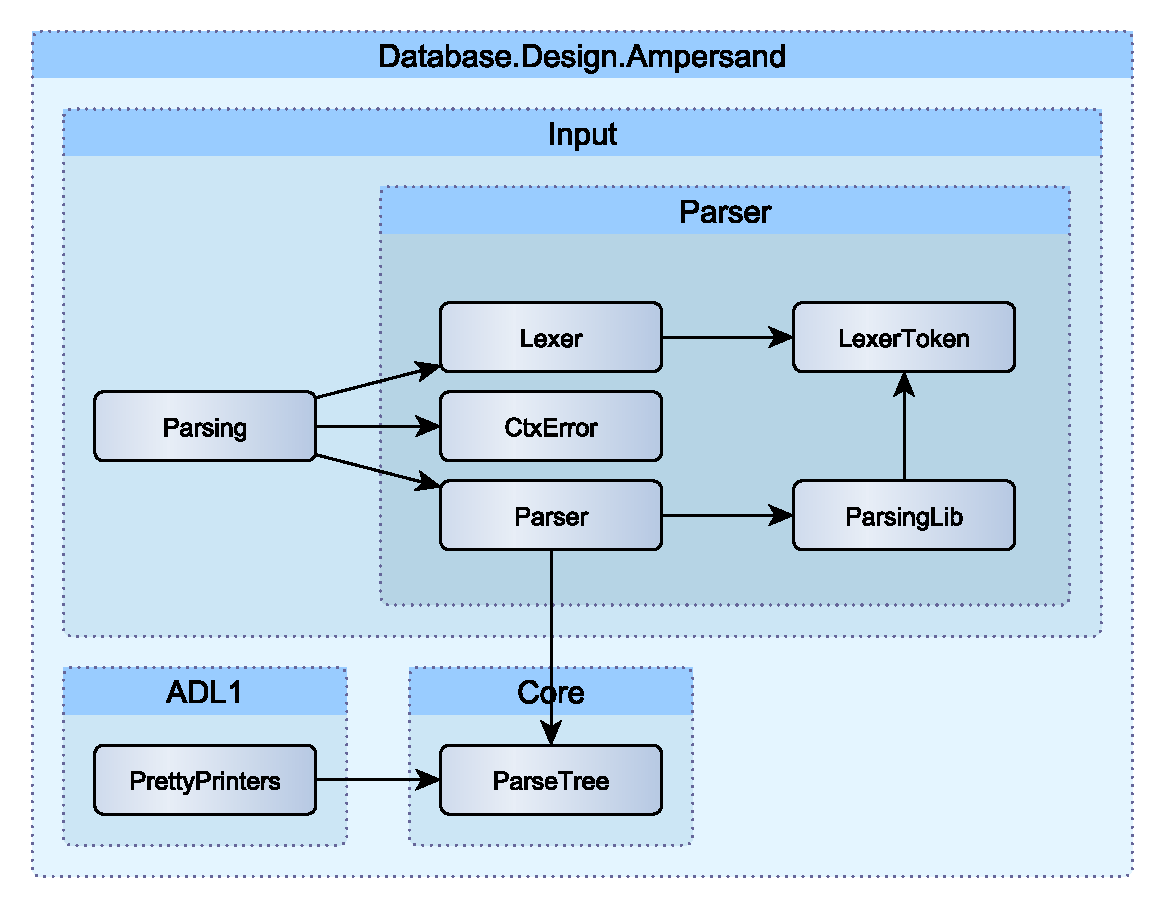
\includegraphics[width=0.7\columnwidth]{Figures/ParserModules}
    \caption{The modules relevant for the parser and their dependencies}
    \label{fig:ParserModules}
  \end{figure}%

  The parsing process starts in the module \code{Parsing}.
  As a first step, the input string is sliced into tokens by the \code{lexer} module.
  Once the input string is separated into the token structure as defined in the module \code{LexerToken} the next step is to actually parse the tokens by the \code{Parser}.
  The parser will use the \code{ParsingLib} to create the parse tree as defined in \code{ParseTree}.

  ~\\\noindent
  Each main module has the following responsibilities:
  %
  \begin{description}
    \item[Parsing] module that implements the interface of the parser with the rest of the system.
      It is responsible for reading the input files, calling the lexer and the parser and returning a parse tree as result (or a parse error).

    \item[Lexer/LexerToken] modules responsible for recognizing the input characters and converting them to tokens.
      The new lexer, together with its sub-modules, splits the input strings into the token structure defined in \code{LexerToken}.
      This list of tokens is the actual input for the parser.

    \item[Parser] module responsible for executing the parsing itself.
      It accepts the tokens that are allowed in each grammar production and generates the corresponding parse tree.
      The parser is described in \autoref{design:new-parser}.
 \end{description}

  \noindent
  Several supporting modules are defined used by one or more main modules:
  \begin{description}
    \item[ParsingLib] library that contains several useful functions to assist the parser, e.g. token recognition.
      These functions are not depending on the specific grammar rules.
      
    \item[ParseTree] external module containing the parse tree data structures.
      Only details of this module have been changed during this project (e.g. field ordering).
    
    \item[PrettyPrinters] contains instances of the \code{Pretty} type class for the parse tree data types and the functions responsible for printing the parse tree to ADL scripts in a `pretty' way.

    \item[CtxError] contains the data structures responsible for the parse errors and their location.
      This module has not been refactored as a part of this project.
    
  \end{description}

% !TEX root = ../Thesis.tex

\subsection{Sofware Quality Factors (M)}
\label{results:software-quality}
% Maintainability

\subsubsection{Documentation}
\lipsum[2]
% Haddock + EBNF comments

\subsubsection{Readability}
\lipsum[4]
% HLint + Shorter code + refactorings

\subsubsection{Performance}
\lipsum[5]
% Efficiency
% !TEX root = ../Thesis.tex

\subsection{New Lexer: The rationale behind the new lexer}
\label{subsec:newlexer}

In the design of the new Ampersand parser, the question arose whether to keep the current scanner, the former name of the lexer module within Ampersand, or to implement a new one.
After the analysis of the error improvement areas, as described in \autoref{sec:analysis}, the main improvements were identified within the actual parser.
The error feedback quality produced by the scanner module was higher and therefore, there was no stringent need to re-implement the scanner.
On the other hand, given the aspect that Parsec was defined as the new parser library, keeping the current scanner would have resulted in the utilization of two different libraries providing more of less the same functionality.
To avoid a decrease in maintainability, the decision is made to implement the parser and scanner based on the same library.

During the implementation of the lexer module, replacing the old scanner, additional attention was given to further improve the quality of the error messages.
The scanner module is renamed to lexer to stress the aspect that the principle of lexemes is used in the new scanner.
Lexemes can be seen as the part of a token containing the actual language content besides the actual position information.

The lexer is built based on the existing Helium lexer modules. 
Helium is a Haskell compiler with the main goal of giving user friendly error messages \citeac{helium}.
The lexer module in Helium contains interesting principles such as position monitoring, warnings and easy maintainable error messages.
% !TEX root = ../Thesis.tex

\subsection{Lexer}
\label{analysis:lexer}
The lexer module is responsible to split up the input stream into tokens.
Tokens are meaningful pieces of the input string that can be recognized by the parser.

The following improvement points were identified after analysis:
\begin{description}
  \item[Dispersed error messages]
    The error messages produced by the lexer are of good quality.
    Each error message is however defined directly within the corresponding lexer function making the maintenance harder.
  \item[Complex token structure]
    The token structure is complex and confusing.
    Two values are present in the token, of which one \texttt{val1} is never used.
    There is no distinction between the values used to identify the content of the token and the ones to determine the position of the token.
  \item[Module structuring]
    In the lexer, the actual lexing functions are intermingled with data types, supporting functions and error message texts.
    This makes the lexer hard to understand and to maintain.
  \item[Language support]
    The errors are returned in English only, no multilingual support is available.
  \item[No support for warnings]
    The lexer can only return errors, warnings are not supported. 
  \item[Strings only]
    Token values are stored as strings for all types, with no conversion of integer values.
  \item[Lacking documentation]
    There was no documentation available on how the lexer was designed and structured.
\end{description}


\subsubsection{Token structure}
The old token has the following structure:

\begin{verbatim}
data Token = Tok { tp' :: TokenType
                 , val1 :: String
                 , val2 :: String
                 , pos :: !Pos
                 , file :: !Filename
                 }

data TokenType
  = TkSymbol
  | TkVarid
  | TkConid
  | TkKeyword
  | TkOp
  | TkString
  | TkExpl
  | TkAtom
  | TkChar
  | TkInteger8
  | TkInteger10
  | TkInteger16
  | TkTextnm
  | TkTextln
  | TkSpace
  | TkError
  deriving (Eq, Ord)
\end{verbatim}
%
The arguments have the following purpose:
\begin{description}
  \item[TokenType]
    Identification of the token type. %, i.e. \texttt{TkSymbol}, \texttt{TkVarid}, \texttt{TkConid}, \texttt{TkKeyword}, \texttt{TkOp}, \texttt{TkString}, \texttt{TkExpl}, \texttt{TkAtom}, \texttt{TkChar}, \texttt{TkInteger8}, \texttt{TkInteger10}, \texttt{TkInteger16}, \texttt{TkTextnm}, \texttt{TkTextln}, \texttt{TkSpace} or \texttt{TkError}.
  \item[val1]
    This string argument is not used in the lexer.
    In the case of a \texttt{keyToken} creation, the value is filled in, but we could not find any purpose for this argument.
  \item[val2]
    The actual token content, stored as a string, including the integer values.
  \item[pos]
    Line and column number.
  \item[file]
     Filename in which the token is located.
\end{description}

% !TEX root = ../Thesis.tex

\subsection{New parser}
\label{design:new-parser}
The high-level design of the new parser has not changed much.
While the new parser may still be recognizable for the Ampersand developers, several improvements have been made.

As decided during the research for domain and techniques (see \autoref{domain:parsing}), the parser has been rebuilt with the Parsec combinator library.
Basically, each EBNF rule receives its own parser function.
Thanks to the combinator operators, each parsing function also looks very similar to its corresponding EBNF.

The applicative interface is consistently used.
By changing details of the implementation, e.g. the order of the fields in the parse tree, we have made many of the `rebuild' functions unnecessary.
For some parsers the amount of changes necessary in order to remove supporting functions was too large or even impossible with the current parse tree.

Note that in parts of the parser, the function syntax has substituted the record syntax for creating data objects.
This was done only when the code readability could be improved by doing so.

\subsubsection{Parsec}
\label{design:parsing-lib}
As mentioned earlier, and described in the research context document \citenac{parsing}, the new Ampersand parser has been rebuilt with another parsing library, namely Parsec.
However, for the Ampersand developers, the source code of the parser will still look very familiar, thanks to the applicative interface.
For developers, the main differences between Parsec and the uulib are:
\begin{itemize}
  \item Parsec does not backtrack by default.
    In order to enable backtracking, the \code{try} function must be used.
    This is described in \autoref{design:backtracking}.
  \item Parsec does not try to solve parsing errors.
    The parser stops immediately after the first issue.
   This way, the user is not overwhelmed with irrelevant information.
    See also the error analysis in \autoref{tests:errors}.
  \item Error messages are customizable by using the \code{<?>} operator.
    This is also suggested in \autoref{sec:recommendations}.
  \item Some combinators have a different name, e.g. one must use \code{option} instead of \code{opt}.
    Because the documentation found on Hackage is clear and sufficient, interface differences are not documented here.
\end{itemize}

\subsubsection{Backtracking}
\label{design:backtracking}
In order to explain the differences on backtracking behavior between the uulib and Parsec, we quote here Doaitse Swierstra, the author of the uulib \citenac{swierstra-parsec}:
\begin{quote}
\textsl{%
  To understand the subtleties it is important to understand the differences between the try construct in Haskell and the non-greedy parsing strategy used in uu-parsinglib.
  Effectively the latter is a try which just looks ahead one symbol.
  In that respect it is less powerful than the \code{try} construct from Parsec, in which you specify that a specific construct has to be present completely.
  And then there is the underlying different overall strategy.
  Parsec uses a back-tracking strategy with explicit tries to commit, whereas uu-parsinglib uses a breadth-first strategy with an occasional single symbol look-ahead.
}
\end{quote}
Although the \code{try} construct for backtracking in Parsec is very powerful, it is also undesirable:
Backtracking increases the parser's memory usage, speed, maintainability and the quality of the error messages \citeac{parsec}.
However, they are necessary when the grammar is not left-factored \citeac{parsec}.
In this section we explain why each of the remaining try statements are necessary, and how these issues can be resolved:
\begin{description}
  \item[Classify]
    This ambiguity in the grammar arises from the \code{Classify} and \code{GenDef} productions:
    \begin{ebnf}
     Classify ::= `CLASSIFY' ConceptRef `IS' Cterm
     GenDef ::= (`CLASSIFY' | `SPEC') ConceptRef `ISA' ConceptRef\end{ebnf}
    When the parser encounters \code{`CLASSIFY'}, it cannot determine whether it found a \code{Classify} or a \code{GenDef} production.
    Therefore, the parser must consume the keyword and a \code{ConceptRef} before consuming either \code{`IS'} or \code{`ISA'} and determining which production is applicable.
    
    In order to solve this issue, one must choose a different keyword or symbol for each of the productions.
    Another option would be to merge the two statements in the same parser.
    We did not merge the productions because that would make the parser less maintainable.
  
  \item[Role]
    This ambiguity in the grammar arises from the \code{RoleRelation} and \code{RoleRule} productions:
    \begin{ebnf}
     RoleRelation ::= `ROLE' RoleList `EDITS' NamedRelList
     RoleRule ::= `ROLE' RoleList `MAINTAINS' ADLidList\end{ebnf}
    When the parser encounters \code{`ROLE'}, it cannot determine whether it is a \code{RoleRelation} or a \code{RoleRule} production.
    Therefore, the parser must consume the keyword and a \code{RoleList} (which may be long) before consuming either \code{`MAINTAINS'} or \code{`EDITS'} and determining which production is applicable.
    
    In order to solve this issue, one must choose a different keyword for each of the productions, merge the two options to have the same representation in the parse tree, or refactor the parser so that the two options are parsed together.
    We did not merge the productions because that would make the parser less maintainable.
  
  \item[View]
    This ambiguity in the grammar arises from the \code{FancyViewDef} and \code{ViewDefLegacy} productions:
    \begin{ebnf}
     FancyViewDef ::= `VIEW' Label ConceptOneRefPos `DEFAULT'? `{' ViewObjList `}' HtmlView? `ENDVIEW'
     ViewDefLegacy ::= (`VIEW' | `KEY') LabelProps ConceptOneRefPos `(' ViewSegmentList `)'\end{ebnf}
    When the parser encounters \code{`VIEW'}, it cannot define whether it found a \code{FancyViewDef} or a \code{ViewDefLegacy} production.
    In this case, defining which construction is applicable is even more complicated.
    This decision must, in the worst case, be delayed until the parser encounters a \code{`\{'} or \code{'('}.
    That is because the productions \code{Label} and \code{LabelProps} are not disjoint, and \code{`DEFAULT'} is optional.
    
    In order to solve this issue, we advise to merge or drop the legacy statement.
    
  \item[Multiplicity]
    This ambiguity in the grammar arises from the \code{Mult} production:
    \begin{ebnf}
     Mult ::= (`0' | `1') `..' (`1' | `*') | `*' | `1'\end{ebnf}
    When the parser encounters \code{`1'}, it cannot define whether it found the first or the last production.
    The parser must therefore read the next token before choosing the right option.
    
    In order to solve this issue, we advise to refactor the grammar (and the parser) to have the following production:
    \begin{ebnf}
     Mult ::= `0' `..' (`1' | `*') | `1'(`..' (`1' | `*'))? | `*'\end{ebnf}
    %
    We did not refactor the code in this manner because the \code{pMult} parser does more than only parsing: it also changes the representation of the found constructions before creating the parse tree.
  
  \item[Labels and Terms]
    In two of the productions of the grammar, an ambiguity arises when an optional \code{Label} production is followed by a \code{Term} production (\code{Label? Term}).
    The issue is that \code{Label}, \code{LabelProps}, \code{Rule} and \code{Term} may all begin with a \code{Varid}:
    \begin{ebnf}
     Label ::= ADLid `:' => Varid `:'
     LabelProps ::= ADLid (`{'ADLidListList`}')? `:' => Varid `:'
     Rule ::= Term (`=' Term | `|-' Term)? => Term
     Term => Trm2 => Trm3 => Trm4 => Trm5 => Trm6 => RelationRef => NamedRel => Varid Sign?\end{ebnf}
    %
    This ambiguity exists in the \code{Att} and \code{RuleDef} productions:
    \begin{ebnf}
     Att ::= LabelProps? Term
     RuleDef ::= `RULE' Label? Rule Meaning* Message* Violation?\end{ebnf}
    
    What happens here is that when the parser encounters a \code{Varid}, it cannot define whether it is part of the (optional) \code{Label} production or if no \code{Label} was given and the \code{Varid} is part of a \code{Term}/\code{NamedRel} production.
    
    Due to the quite complex grammar for the \code{Term} production, this issue may severely impact the parser's performance.
    This is probably the most harmful of the ambiguities mentioned.
    However, it can only be solved by adding a symbol before the \code{Term} production (e.g. making the `:' non-optional).
\end{description}
%
Please note that in order to have proper backtracking with correct error messages, Parsec may require two try-statements \citenac{try-harmful}.

\subsubsection{Changes to the parse tree}
\label{design:parse-tree}
Improvements in the Ampersand parse tree are out of the scope of this project, because of the potential consequences to the rest of the Ampersand system.
However, during the development of the new parser a few constructions have been changed in order to make the parser more readable and maintainable.
The changes have been mostly in the order of the constructor parameters, and this was done consequently though all Ampersand modules.
The updated parse tree is depicted in the \hyperref[app:docs]{project documentation (appendix)}.

% !TEX root = ../Parsing.tex

\section{User-friendly error messages}
\label{sec:errors}
The most important feature of the parser that will be built, is that it should generate user-friendly error messages.
To understand what kinds of messages can be (and should be) generated, a research will be done on what good errors are and how to generate them.

This is also related to the choice of the parsing library, since the chosen library should support the generation of good errors without extensive effort.
Coincidently, a good source of knowledge are the papers of the supervisor, Bastiaan Heeren, who has done his PhD thesis on the generation of top quality type error messages\cite{heeren-error}.

% !TEX root = ../Documentation.tex

\subsection{Next steps (M)}
\label{subsec:design-next-steps}

During the parser re-implementation and code re-factoring to enhance the code maintainability, we noticed potential improvement topics in Ampersand.
Were possible, with respect to our project requirements and our milestones, we integrated these topics in the new parser.
Some topics we could not handle due to time constraints or given the undesired impact on the surrounding modules.
It would be a pity if these improvement ideas were lost as these can help the Ampersand team to further enhance the tool.
This section summarizes our improvement suggestions, both generic as specific ones, for the Ampersand tool.

\begin{description}
  \item[Syntax improvements]
    In the syntax, we discovered some statements which are not pure LL(k) statements.
    The Parsec \texttt{try} function allows the backtracking in the parser, avoiding that input is consumed which is still needed in another parse statements if the parse function can not succeed successfully.
    Using \texttt{try} we can handle this situation but the backtracking has a negative impact of the parser performance whilst it adds complexity to the parser module. 
    Our suggestion is to further optimize the Ampersand syntax to establish a pure predictive syntax in which no backtracking is needed.
    This will not only improve the parser performance and maintainability, the syntax simplifications will .
    The syntax statements in which backtracking is needed, including the reasons why, are listed in section \autoref{subsec:backtracking}.

  \item[Warnings]
    An improvement point in the new lexer is that warnings are now supported. 
    Warnings are however not yet integrated in the Ampersand tool.
    There is no need to stop the compiling process for warnings, as the reasons behind them can make sense.
    Warnings can, however, support the user identifying the cause of unexpected results, although the compilation could be completed successfully.
    Our suggestion is to add the list of warnings to the design artifacts of Ampersand, available for the user to reflect on is needed.

  \item[Uniform parse tree structure]

todo


  \item[Manual overrule of error message]
    Our analysis of the new error messages showed that the quality of these improved distinctively.
    Parsec provides to possibility to overrule the standard Parsec error message by an own formulated message.
    During our implementation we decided to stick to the standard if the standard error message was, at least, sufficient.
    If the Ampersand teams want to tweak some error message after all, this can be realized using the \texttt{<?>} Parsec function.
    Placing the \texttt{<?>} after the parser, followed by a string, changes the standard Parsec text after the keyword `expecting'.

\end{description}


\newpage
% !TEX root = ../Thesis.tex

\section{Test Report}
\label{sec:tests}

% !TEX root = ../Thesis.tex

\subsection{Test suite}
  Together with the new parser, a test suite has been developed.
  This test suite has been used to verify the performance and correctness of the new parser.
  The source code can be found in the folder \code{src/Database/Design/Ampersand/Test} within the Ampersand repository.

  The test suite runs in three steps (see \autoref{fig:TestModules}).
  The first step is to check if a list of input files can be parsed successfully. 
  If no issues are found during the parsing, the same list is used by the module \code{RunAmpersand} in which all input scripts are processed completely by Ampersand.
  As a final step, a series of random generated parse tree structures is generated, translated in ADL files and tested.
  Each of the modules are described in the following subsection.
  %
  \begin{figure}[ht]%
    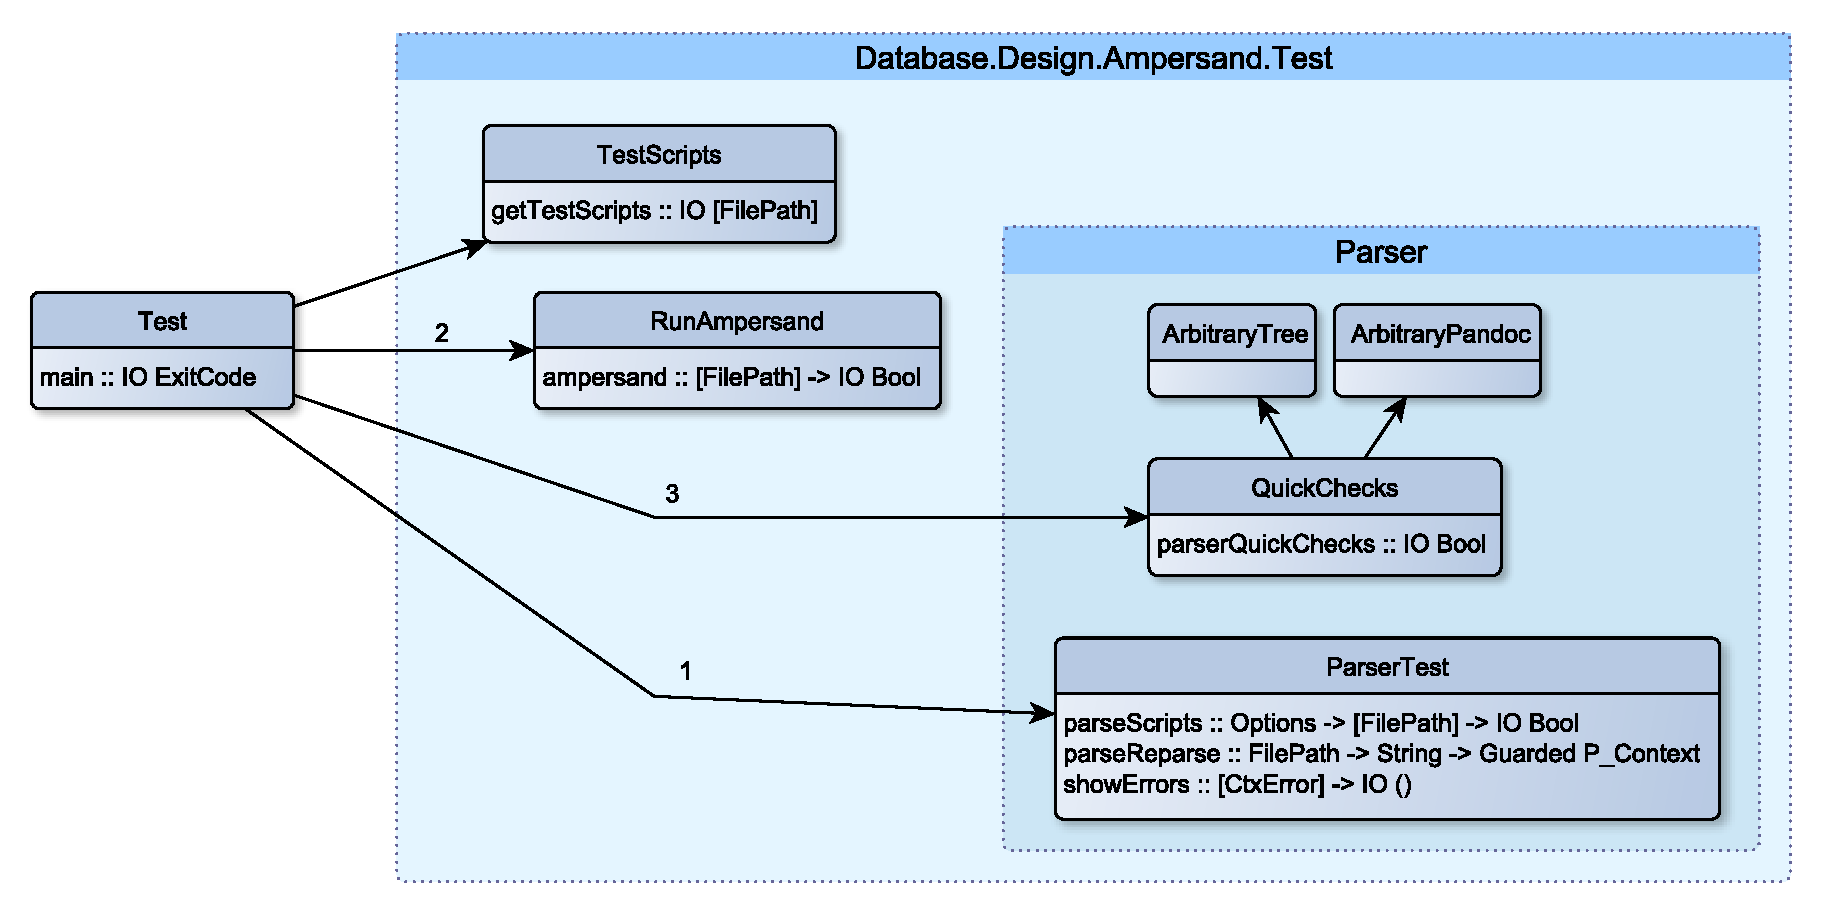
\includegraphics[width=\columnwidth]{Figures/TestModules}
    \caption{Test suite modules with their exported functions}
    \label{fig:TestModules}
  \end{figure}%

  %todo: herwerking op basis van de opmerkingen van Bastiaan
  \subsubsection{Modules}
  \label{tests:test-modules}
  In this section a short description of each module is given:%
  %
  \begin{description}
    \item[Test] contains the \code{main} method that can be executed to run the test suite.
      The \code{main} function calls each of the other modules in sequence, stopping if any of them returns \code{False}.
      When all tests have been successful, the return code is \code{ExitSuccess}.
      Otherwise, the return code is naturally \code{ExitFailure}.
	  
    \item[ParserTest] exports three functions that are the core of testing the parser:
      \begin{itemize}
        \item \code{parseScripts} receives a list of files to parse, and checks that every file can be parsed successfully.
        \item \code{parseReparse} tries to parse a file, and if successful, pretty-prints the result and parses it again.
        \item \code{showErrors} prints the given parse errors to the output.
      \end{itemize}
    
    \item[RunAmpersand] receives a list of files, and checks that every file can be executed successfully by Ampersand.
      This tests thus not only the parser, but also the interface between the parser and the type checker, as the rest of the Ampersand chain.
  \end{description}
	  
  The following modules are supporting one ore more of the three main modules:
  \begin{description}	  
    \item[TestScripts] retrieves a list of scripts that can be used for the different tests.
      It searches for tests within the folder \code{ArchitectureAndDesign}, and contains a list of scripts from the \code{ampersand-models} repository, that can be changed at a later moment if wished.
      Note that all the ADL-scripts listed in this section must be correct for the parser and the type checker.
      During development, the list was limited to the scripts that could be successfully executed by the original Ampersand version.   
	  
    \item[QuickChecks] generates random parse tree structures and generates the corresponding ADL-script by pretty printing the parse tree.
      This ADL-script is then fed back to the parser through the \code{parseReparse} function, to verify that the parser can accept any random input.
      More information on the quick checks is given in subsection~\ref{tests:quick-check}.
    
    \item[ArbitraryTree] is a support module that gives \code{Arbitrary} instances to all parse-tree structures.
      This is used by QuickCheck as described in subsection~\ref{tests:quick-check}.
    
    \item[ArbitraryPandoc] contains \code{Arbitrary} instances to the Pandoc data types.
      This file has not been developed in this project, but copied from the \code{jgm/pandoc} project with the GPL license.
  \end{description}

  \subsubsection{QuickCheck and pretty printing}
  \label{tests:quick-check}
  The most innovative part of the test suite is the use of random structures to test the parser.
  In this section we describe how this generation is implemented.
  
  The main role in the generation of random structures is played by the support library QuickCheck, which has been added to the Ampersand project.
  QuickCheck is able to generate any data structure randomly.
  However, since the parse tree is a custom structure that must obey specific rules, QuickCheck requires the specification of these rules by instances of the \code{Arbitrary} class.
  
  Every data structure in the parse tree has received an \code{Arbitrary} instance used for test purposes.
  The instances can be found in the module \code{Database.Design.Ampersand.Test.Parser\-.ArbitraryTree}, as described in subsection~\ref{tests:test-modules}.
  
  After generating the random parse trees, the test suite needs to convert them to ADL-scripts.
  The conversion of parse tree to source code is also known as pretty printing.
  As the pretty printing is seen as part of the parse tree, it is not included in the Test modules, but is part of the input subsystem.
  The pretty printing instances are found in the module \code{Database.Design.Ampersand.ADL1.PrettyPrinters}.
  This module makes use of the library \code{Text.PrettyPrint.Leijen}, that outlines the output so it is indeed `pretty'.
  
  Now that the ADL source is available, the parser is executed.
  The result of the parser is checked to be equal to the generated tree by the property \code{prop\_pretty}.
  The property is currently tested for 64 generated parse trees in the test suite.
  If the test fails for any generated structure, the test suite fails with an appropriate error.
  
  \subsubsection{Running the tests}
  During the parser development, the \code{main} function of the parser tests has been executed manually, through a batch file.
  This is mainly done because the project team did not have access to the Sentinel server, and no documentation was available on how to run Sentinel locally on a Windows machine.
  However, now that the parser is being delivered, it should be integrated with the other existing Ampersand/Sentinel tests.
  We leave the option open for the Ampersand development team to either add the Sentinel jobs to this test suite, or to add the parser test suite to the Sentinel jobs.
  
  \subsubsection{Test coverage}
  %TODO: Update the numbers when delivery is ready.
  The main objective of the test suite is naturally to test the parser.
  By using HPC (Haskell Program Coverage) we verified that the most important parts of the code were well tested.
  For instance, the \code{Parser} module is covered by 96\%.
  \code{ParsingLib} is 87\% covered, while the module \code{Lexer} is 82\% tested.
  Finally, the module \code{PrettyPrinters} is 98\% covered.
  The complete list with the code coverage is available in the generated HPC report, which is part of the \hyperref[app:docs]{project documentation (appendix)}.
  
  Note that the parts of the code that were not tested, could not be tested for two reasons: only valid ADL files are tested automatically; the incorrect files are tested manually (see \autoref{tests:errors}).
  The other reason is that the ADL files provided did not contain all possible grammar constructions.
  Given the extend to which the errors are tested manually we believe that the full test coverage will be very close to 100\%.
  
% !TEX root = ../Parsing.tex

\section{User-friendly error messages}
\label{sec:errors}
The most important feature of the parser that will be built, is that it should generate user-friendly error messages.
To understand what kinds of messages can be (and should be) generated, a research will be done on what good errors are and how to generate them.

This is also related to the choice of the parsing library, since the chosen library should support the generation of good errors without extensive effort.
Coincidently, a good source of knowledge are the papers of the supervisor, Bastiaan Heeren, who has done his PhD thesis on the generation of top quality type error messages\cite{heeren-error}.

\newpage
% !TEX root = ../Thesis.tex

% overzicht van alle topics, samengevat waar mogelijk, die nog als todo staan of waar we verdere verbertering voorstellen
\section{Recommendations}
\label{sec:recommendations}
Although we believe the new parser is a large step forward, we also recognize that there are still improvements to be made.

Ampersand is growing and changing in a fast pace.
This is a direct consequence of a project involved with research and active development.
In such projects, it is often impossible to predict which functionalities will be necessary and to design the domain-specific language accordingly beforehand.

As expected we see that most of the remaining issues are related to the grammar ambiguities that force backtracking.
Also the parse tree is not consistently designed.
These issues are mentioned in \autoref{recommendations:design}.
Other improvements are also possible in the test framework delivered.
Those are mentioned in \autoref{recommendations:tests}.

% !TEX root = ../Documentation.tex

\section{Design}
\label{sec:design}
% !TEX root = ../Documentation.tex

\subsection{System overview}
\label{design:system-overview}
  The parser module overview is given in \autoref{fig:ParserModules}.
  \begin{figure}[ht]%
    \centering
    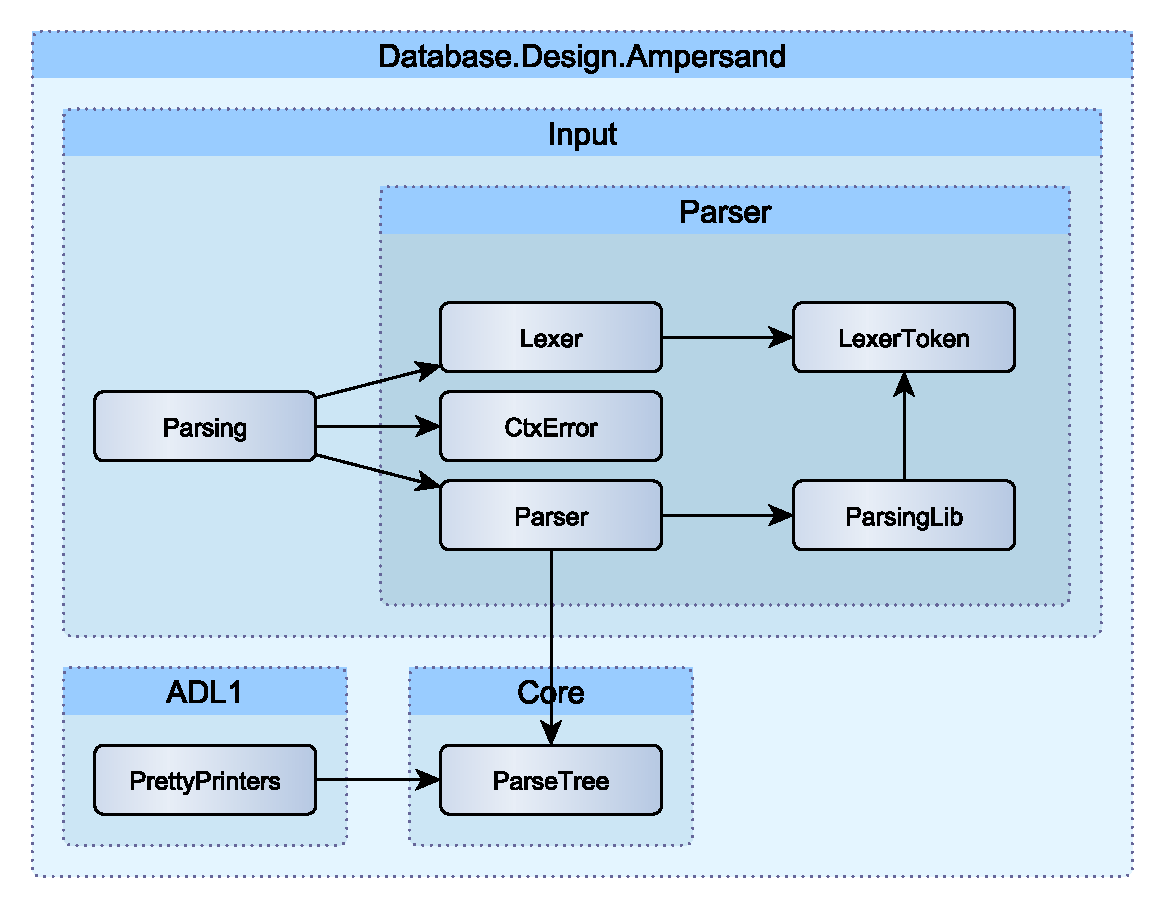
\includegraphics[width=0.7\columnwidth]{Figures/ParserModules}
    \caption{The modules relevant for the parser and their dependencies}
    \label{fig:ParserModules}
  \end{figure}%

  The parsing process starts in the module \code{Parsing}.
  As a first step, the input string is sliced into tokens by the \code{lexer} module.
  Once the input string is separated into the token structure as defined in the module \code{LexerToken} the next step is to actually parse the tokens by the \code{Parser}.
  The parser will use the \code{ParsingLib} to create the parse tree as defined in \code{ParseTree}.

  ~\\\noindent
  Each main module has the following responsibilities:
  %
  \begin{description}
    \item[Parsing] module that implements the interface of the parser with the rest of the system.
      It is responsible for reading the input files, calling the lexer and the parser and returning a parse tree as result (or a parse error).

    \item[Lexer/LexerToken] modules responsible for recognizing the input characters and converting them to tokens.
      The new lexer, together with its sub-modules, splits the input strings into the token structure defined in \code{LexerToken}.
      This list of tokens is the actual input for the parser.

    \item[Parser] module responsible for executing the parsing itself.
      It accepts the tokens that are allowed in each grammar production and generates the corresponding parse tree.
      The parser is described in \autoref{design:new-parser}.
 \end{description}

  \noindent
  Several supporting modules are defined used by one or more main modules:
  \begin{description}
    \item[ParsingLib] library that contains several useful functions to assist the parser, e.g. token recognition.
      These functions are not depending on the specific grammar rules.
      
    \item[ParseTree] external module containing the parse tree data structures.
      Only details of this module have been changed during this project (e.g. field ordering).
    
    \item[PrettyPrinters] contains instances of the \code{Pretty} type class for the parse tree data types and the functions responsible for printing the parse tree to ADL scripts in a `pretty' way.

    \item[CtxError] contains the data structures responsible for the parse errors and their location.
      This module has not been refactored as a part of this project.
    
  \end{description}

% !TEX root = ../Thesis.tex

\subsection{Lexer}
\label{analysis:lexer}
The lexer module is responsible to split up the input stream into tokens.
Tokens are meaningful pieces of the input string that can be recognized by the parser.

The following improvement points were identified after analysis:
\begin{description}
  \item[Dispersed error messages]
    The error messages produced by the lexer are of good quality.
    Each error message is however defined directly within the corresponding lexer function making the maintenance harder.
  \item[Complex token structure]
    The token structure is complex and confusing.
    Two values are present in the token, of which one \texttt{val1} is never used.
    There is no distinction between the values used to identify the content of the token and the ones to determine the position of the token.
  \item[Module structuring]
    In the lexer, the actual lexing functions are intermingled with data types, supporting functions and error message texts.
    This makes the lexer hard to understand and to maintain.
  \item[Language support]
    The errors are returned in English only, no multilingual support is available.
  \item[No support for warnings]
    The lexer can only return errors, warnings are not supported. 
  \item[Strings only]
    Token values are stored as strings for all types, with no conversion of integer values.
  \item[Lacking documentation]
    There was no documentation available on how the lexer was designed and structured.
\end{description}


\subsubsection{Token structure}
The old token has the following structure:

\begin{verbatim}
data Token = Tok { tp' :: TokenType
                 , val1 :: String
                 , val2 :: String
                 , pos :: !Pos
                 , file :: !Filename
                 }

data TokenType
  = TkSymbol
  | TkVarid
  | TkConid
  | TkKeyword
  | TkOp
  | TkString
  | TkExpl
  | TkAtom
  | TkChar
  | TkInteger8
  | TkInteger10
  | TkInteger16
  | TkTextnm
  | TkTextln
  | TkSpace
  | TkError
  deriving (Eq, Ord)
\end{verbatim}
%
The arguments have the following purpose:
\begin{description}
  \item[TokenType]
    Identification of the token type. %, i.e. \texttt{TkSymbol}, \texttt{TkVarid}, \texttt{TkConid}, \texttt{TkKeyword}, \texttt{TkOp}, \texttt{TkString}, \texttt{TkExpl}, \texttt{TkAtom}, \texttt{TkChar}, \texttt{TkInteger8}, \texttt{TkInteger10}, \texttt{TkInteger16}, \texttt{TkTextnm}, \texttt{TkTextln}, \texttt{TkSpace} or \texttt{TkError}.
  \item[val1]
    This string argument is not used in the lexer.
    In the case of a \texttt{keyToken} creation, the value is filled in, but we could not find any purpose for this argument.
  \item[val2]
    The actual token content, stored as a string, including the integer values.
  \item[pos]
    Line and column number.
  \item[file]
     Filename in which the token is located.
\end{description}

% !TEX root = ../Thesis.tex

\subsection{New Parser}
\lipsum[5]
% !TEX root = ../Thesis.tex

\subsection{Parse tree (R-M)}
\label{analysis:parse-tree}
The parse tree (also known as P-structure) is a data structure that very much resembles the EBNF description.
The root of the tree is the \code{P\_Context} structure, and every leaf of the tree has a field for the location where it was found in the ADL code (the \code{Origin} structure).
The tree is consistently defined with the record syntax and is well documented.

However, the constructions are not completely pure, since some transformations are necessary from the ADL to the P-structure.
This forces the parser to do more than only parsing.
Also, the order of the fields can be confusing; sometimes \code{Origin} is the first field and sometimes it is not.

During this project, small changes to the parse tree have been done.
These changes are described in \autoref{design:parse-tree}.

% !TEX root = ../Parsing.tex

\section{User-friendly error messages}
\label{sec:errors}
The most important feature of the parser that will be built, is that it should generate user-friendly error messages.
To understand what kinds of messages can be (and should be) generated, a research will be done on what good errors are and how to generate them.

This is also related to the choice of the parsing library, since the chosen library should support the generation of good errors without extensive effort.
Coincidently, a good source of knowledge are the papers of the supervisor, Bastiaan Heeren, who has done his PhD thesis on the generation of top quality type error messages\cite{heeren-error}.

% !TEX root = ../Documentation.tex

\subsection{Next steps (M)}
\label{subsec:design-next-steps}

During the parser re-implementation and code re-factoring to enhance the code maintainability, we noticed potential improvement topics in Ampersand.
Were possible, with respect to our project requirements and our milestones, we integrated these topics in the new parser.
Some topics we could not handle due to time constraints or given the undesired impact on the surrounding modules.
It would be a pity if these improvement ideas were lost as these can help the Ampersand team to further enhance the tool.
This section summarizes our improvement suggestions, both generic as specific ones, for the Ampersand tool.

\begin{description}
  \item[Syntax improvements]
    In the syntax, we discovered some statements which are not pure LL(k) statements.
    The Parsec \texttt{try} function allows the backtracking in the parser, avoiding that input is consumed which is still needed in another parse statements if the parse function can not succeed successfully.
    Using \texttt{try} we can handle this situation but the backtracking has a negative impact of the parser performance whilst it adds complexity to the parser module. 
    Our suggestion is to further optimize the Ampersand syntax to establish a pure predictive syntax in which no backtracking is needed.
    This will not only improve the parser performance and maintainability, the syntax simplifications will .
    The syntax statements in which backtracking is needed, including the reasons why, are listed in section \autoref{subsec:backtracking}.

  \item[Warnings]
    An improvement point in the new lexer is that warnings are now supported. 
    Warnings are however not yet integrated in the Ampersand tool.
    There is no need to stop the compiling process for warnings, as the reasons behind them can make sense.
    Warnings can, however, support the user identifying the cause of unexpected results, although the compilation could be completed successfully.
    Our suggestion is to add the list of warnings to the design artifacts of Ampersand, available for the user to reflect on is needed.

  \item[Uniform parse tree structure]

todo


  \item[Manual overrule of error message]
    Our analysis of the new error messages showed that the quality of these improved distinctively.
    Parsec provides to possibility to overrule the standard Parsec error message by an own formulated message.
    During our implementation we decided to stick to the standard if the standard error message was, at least, sufficient.
    If the Ampersand teams want to tweak some error message after all, this can be realized using the \texttt{<?>} Parsec function.
    Placing the \texttt{<?>} after the parser, followed by a string, changes the standard Parsec text after the keyword `expecting'.

\end{description}


% !TEX root = ../Thesis.tex

% Overzicht van alle mogelijke code verbeteringen die we nog zien
% alle trys worden hierin exhaustief opgenomen
% alle todo's scannen en aanbevelen waar syntaxt optimalisatie hier kan helpen

\subsection{Syntax (M)}
\lipsum[1]

% !TEX root = ../Thesis.tex

% besprekingvan alle mogelijke code verbeteringen die we door ene impact op de parse tree of andere redenen niet behandeld hebben

\subsection{Coding (R-D)}
In the actual parser code, some smaller improvement topics are identified.
Resolving these independent minor topics impacts however the parse tree and therefore, these modifications are still open.
providing a exhaustive overview of these topics in this document would jeopardize the briefness and conciseness of this document.
All improvement topics are however fully documented in the code itself.
% !TEX root = ../Thesis.tex

\section{Test Report}
\label{sec:tests}

% !TEX root = ../Thesis.tex

\subsection{Test suite}
  Together with the new parser, a test suite has been developed.
  This test suite has been used to verify the performance and correctness of the new parser.
  The source code can be found in the folder \code{src/Database/Design/Ampersand/Test} within the Ampersand repository.

  The test suite runs in three steps (see \autoref{fig:TestModules}).
  The first step is to check if a list of input files can be parsed successfully. 
  If no issues are found during the parsing, the same list is used by the module \code{RunAmpersand} in which all input scripts are processed completely by Ampersand.
  As a final step, a series of random generated parse tree structures is generated, translated in ADL files and tested.
  Each of the modules are described in the following subsection.
  %
  \begin{figure}[ht]%
    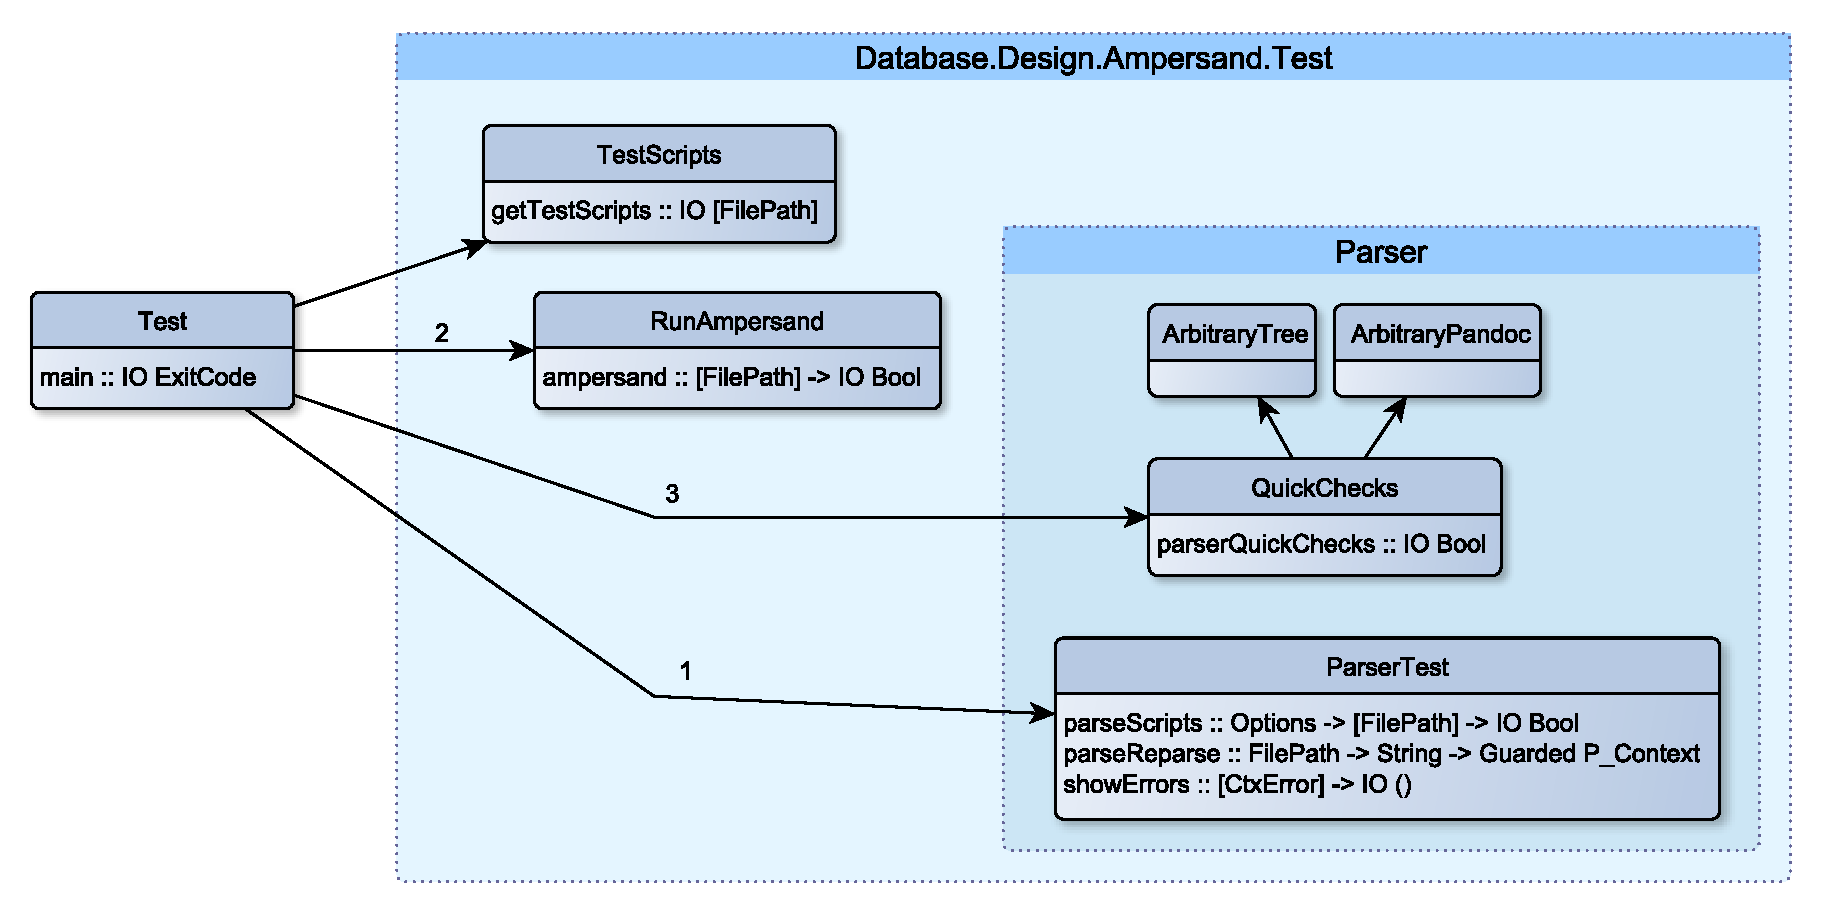
\includegraphics[width=\columnwidth]{Figures/TestModules}
    \caption{Test suite modules with their exported functions}
    \label{fig:TestModules}
  \end{figure}%

  %todo: herwerking op basis van de opmerkingen van Bastiaan
  \subsubsection{Modules}
  \label{tests:test-modules}
  In this section a short description of each module is given:%
  %
  \begin{description}
    \item[Test] contains the \code{main} method that can be executed to run the test suite.
      The \code{main} function calls each of the other modules in sequence, stopping if any of them returns \code{False}.
      When all tests have been successful, the return code is \code{ExitSuccess}.
      Otherwise, the return code is naturally \code{ExitFailure}.
	  
    \item[ParserTest] exports three functions that are the core of testing the parser:
      \begin{itemize}
        \item \code{parseScripts} receives a list of files to parse, and checks that every file can be parsed successfully.
        \item \code{parseReparse} tries to parse a file, and if successful, pretty-prints the result and parses it again.
        \item \code{showErrors} prints the given parse errors to the output.
      \end{itemize}
    
    \item[RunAmpersand] receives a list of files, and checks that every file can be executed successfully by Ampersand.
      This tests thus not only the parser, but also the interface between the parser and the type checker, as the rest of the Ampersand chain.
  \end{description}
	  
  The following modules are supporting one ore more of the three main modules:
  \begin{description}	  
    \item[TestScripts] retrieves a list of scripts that can be used for the different tests.
      It searches for tests within the folder \code{ArchitectureAndDesign}, and contains a list of scripts from the \code{ampersand-models} repository, that can be changed at a later moment if wished.
      Note that all the ADL-scripts listed in this section must be correct for the parser and the type checker.
      During development, the list was limited to the scripts that could be successfully executed by the original Ampersand version.   
	  
    \item[QuickChecks] generates random parse tree structures and generates the corresponding ADL-script by pretty printing the parse tree.
      This ADL-script is then fed back to the parser through the \code{parseReparse} function, to verify that the parser can accept any random input.
      More information on the quick checks is given in subsection~\ref{tests:quick-check}.
    
    \item[ArbitraryTree] is a support module that gives \code{Arbitrary} instances to all parse-tree structures.
      This is used by QuickCheck as described in subsection~\ref{tests:quick-check}.
    
    \item[ArbitraryPandoc] contains \code{Arbitrary} instances to the Pandoc data types.
      This file has not been developed in this project, but copied from the \code{jgm/pandoc} project with the GPL license.
  \end{description}

  \subsubsection{QuickCheck and pretty printing}
  \label{tests:quick-check}
  The most innovative part of the test suite is the use of random structures to test the parser.
  In this section we describe how this generation is implemented.
  
  The main role in the generation of random structures is played by the support library QuickCheck, which has been added to the Ampersand project.
  QuickCheck is able to generate any data structure randomly.
  However, since the parse tree is a custom structure that must obey specific rules, QuickCheck requires the specification of these rules by instances of the \code{Arbitrary} class.
  
  Every data structure in the parse tree has received an \code{Arbitrary} instance used for test purposes.
  The instances can be found in the module \code{Database.Design.Ampersand.Test.Parser\-.ArbitraryTree}, as described in subsection~\ref{tests:test-modules}.
  
  After generating the random parse trees, the test suite needs to convert them to ADL-scripts.
  The conversion of parse tree to source code is also known as pretty printing.
  As the pretty printing is seen as part of the parse tree, it is not included in the Test modules, but is part of the input subsystem.
  The pretty printing instances are found in the module \code{Database.Design.Ampersand.ADL1.PrettyPrinters}.
  This module makes use of the library \code{Text.PrettyPrint.Leijen}, that outlines the output so it is indeed `pretty'.
  
  Now that the ADL source is available, the parser is executed.
  The result of the parser is checked to be equal to the generated tree by the property \code{prop\_pretty}.
  The property is currently tested for 64 generated parse trees in the test suite.
  If the test fails for any generated structure, the test suite fails with an appropriate error.
  
  \subsubsection{Running the tests}
  During the parser development, the \code{main} function of the parser tests has been executed manually, through a batch file.
  This is mainly done because the project team did not have access to the Sentinel server, and no documentation was available on how to run Sentinel locally on a Windows machine.
  However, now that the parser is being delivered, it should be integrated with the other existing Ampersand/Sentinel tests.
  We leave the option open for the Ampersand development team to either add the Sentinel jobs to this test suite, or to add the parser test suite to the Sentinel jobs.
  
  \subsubsection{Test coverage}
  %TODO: Update the numbers when delivery is ready.
  The main objective of the test suite is naturally to test the parser.
  By using HPC (Haskell Program Coverage) we verified that the most important parts of the code were well tested.
  For instance, the \code{Parser} module is covered by 96\%.
  \code{ParsingLib} is 87\% covered, while the module \code{Lexer} is 82\% tested.
  Finally, the module \code{PrettyPrinters} is 98\% covered.
  The complete list with the code coverage is available in the generated HPC report, which is part of the \hyperref[app:docs]{project documentation (appendix)}.
  
  Note that the parts of the code that were not tested, could not be tested for two reasons: only valid ADL files are tested automatically; the incorrect files are tested manually (see \autoref{tests:errors}).
  The other reason is that the ADL files provided did not contain all possible grammar constructions.
  Given the extend to which the errors are tested manually we believe that the full test coverage will be very close to 100\%.
  
% !TEX root = ../Parsing.tex

\section{User-friendly error messages}
\label{sec:errors}
The most important feature of the parser that will be built, is that it should generate user-friendly error messages.
To understand what kinds of messages can be (and should be) generated, a research will be done on what good errors are and how to generate them.

This is also related to the choice of the parsing library, since the chosen library should support the generation of good errors without extensive effort.
Coincidently, a good source of knowledge are the papers of the supervisor, Bastiaan Heeren, who has done his PhD thesis on the generation of top quality type error messages\cite{heeren-error}.

% !TEX root = ../Documentation.tex

\subsection{Website and Wiki (R-D)}
\label{recommendations:website}
During the initiation phase of the project we tried to gather as much information as possible regarding the Ampersand project.
The Ampersand project currently has 2 information sources, a Wiki page and a GitHub page.
The Wiki page focuses on the goals and the practical usage of Ampersand where the GitHub page is more oriented to the Ampersand developers.

We experienced that is was not always easy to find the information we were looking for on these sites.
Some information was outdated or sometimes the link was broken. 
Our suggestion is to have both sites more aligned to each other and to take some time to refresh the current Wiki page.
This will make it easier for new Ampersand users to have a kick-start in the Ampersand world.


\newpage
% !TEX root = ../ResearchContext.tex

\section{Conclusion}
\label{sec:conclusion}
The Ampersand approach is situated within several research contexts, such as the Business Rule Approach and formal systems.
Additionally, the Ampersand Parser is part of a broader parser research context.
Our conclusion is that the new Ampersand parser has a very small influence in its research context for business rules.
This parser does not offer any new features or improvements to the language.
The largest influence of the project is commercial and educational by improving the user experience.
We expect that the new parser will allow commercial, research and educational users to do their work faster and more efficiently.


\newpage

% !TEX root = ../Thesis.tex

\appendix
\addcontentsline{toc}{part}{Appendices}
% !TEX root = ../ResearchContext.tex

\small
\printglossary[style=mcolindex,title=Glossary]
\label{sec:glossary}

\clearpage
% !TEX root = ../Planning.tex
\addcontentsline{toc}{section}{References}
\label{sec:bibliography}

\begin{thebibliography}{99}

%TODO: Check the order of the bibliography

\bibitem{business-rules}
	The Business Rules Manifesto\\
	Version 2.0, November 1, 2003\\
	Ronald G. Ross\\
	\url{http://www.businessrulesgroup.org/brmanifesto.htm}
	
\bibitem{ampersand-approach}
	Ampersand: foutvrije specificaties voor B\&I-vraagstukken\\
	Informatie magazine, August 2007\\
	Stef Joosten, Rieks Joosten and Sebastiaan Joosten\\
	\url{http://informatie.nl/Artikelen/2007/augustus/Default.aspx}  % AmpersandfoutvrijespecificatiesvoorBI-vraagstukken.aspx
	
\bibitem{ampersand-architecture}
	Ampersand Software Architecture\\
	\url{http://wiki.tarski.nl/index.php/Software_Architecture}
	
\bibitem{pmi}
	Project Management Institute\\
	\url{http://www.pmi.org}
	
\bibitem{open-issues}
	Requirements for a parser of Ampersand\\
	Stef Joosten\\
	Version \texttt{8e27daf}, September 25, 2014\\
%	{\footnotesize \url{https://github.com/AmpersandTarski/ampersand/tree/ABI\_Parser/ArchitectureAndDesign}}
	\url{https://github.com/AmpersandTarski/ampersand/commit/8e27daf}
	
\bibitem{ampersand-wiki}
	Ampersand Coding Conventions\\
	Stef Joosten \& Han Joosten\\
	Version 4, September 6, 2011\\
	\url{http://wiki.tarski.nl/index.php/Coding\_conventions}.

\bibitem{heeren-error}
	Top Quality Type Error Messages\\
	Bastiaan Heeren\\
	ISBN 90-393-4005-6, September 20, 2005\\
	\url{www.open.ou.nl/bhr/phdthesis}.
	
\bibitem{iso-9126}
	Software Engineering -- Product quality\\
	International Organization for Standardization\\
	ISO/IEC 9126:2001\\
	\url{http://www.iso.org/iso/iso_catalogue/catalogue_tc/catalogue_detail.htm?csnumber=22749}.

\bibitem{jstd-016}
	J-STD-016 Standard for Software Development and Documentation\\
	Annex F.2.4: Contents of the Software Requirements Specification (SRS)\\
	Department of Defense, United States of America\\
	September 1995\\
	ISBN 0-7381-0427-2, SS94377.

\end{thebibliography}

\end{document}